% paper1_ja.tex  —  v2 (N=120, Ridge regression, C robustness)
% Compile:
%   uplatex paper1_ja.tex && dvipdfmx paper1_ja.dvi
%
% Required files under reports/paper_figs_v2/:
%   fig_permutation_C_bar.png, fig_teacher_heatmap.png, fig_bootstrap_C_radar.png
%   tab_feature_definitions.tex, tab_descriptive_stats.tex, tab_permutation_all.tex

\documentclass[dvipdfmx,11pt,a4paper]{bxjsarticle}

\usepackage[dvipdfmx]{graphicx}
\usepackage{booktabs}
\usepackage{longtable}
\usepackage[dvipdfmx]{hyperref}
\usepackage{amsmath}

\graphicspath{{reports/paper_figs_v2/}}

\title{日本語日常会話における相互行為特徴量の定量化指標の提案\\
——コーパス基本情報およびBig Five性格特性による妥当性検証——}
\author{福原 玄\thanks{筆頭著者．合同会社Lead lea（リーレア）．連絡先: genfukuhara@leadlea.com}
\and 山下 祐一\thanks{国立精神・神経医療研究センター（NCNP）神経研究所 疾病研究第七部}
\and 宗田 卓史\thanks{国立精神・神経医療研究センター（NCNP）}}
\date{\today}

\begin{document}
\maketitle

\begin{abstract}
本研究は，日本語日常会話コーパス（CEJC）から抽出可能な
18の相互行為特徴量——発話タイミング（PG），フィラー（FILL），
相互行為構造（IX），応答型（RESP）——を定量化指標として提案し，
その妥当性をコーパス基本情報およびBig Five性格特性との関連から検証する．
CEJC home2サブセットの高品質会話120件（会話$\times$話者ペア）を対象に，
まず18特徴量の分布特性とカテゴリ内・カテゴリ間の相関構造を記述した．
次に，コーパス基本情報（性別・年齢）との関連分析により，
発話率やフィラー使用率が性別・年齢と有意に関連することを確認し，
特徴量の表面的妥当性を示した．
さらに，4つの大規模言語モデル（LLM）が推定したBig Fiveスコアを外部基準として
Ridge回帰（5-fold CV, subject-wise split）と置換検定（5000回）を適用した結果，
Conscientiousness（C: 誠実性）は4教師中3教師で有意な予測精度を示し
（$r = 0.390$--$0.447$, $p < 0.002$），教師間一致度も$\bar{r} = 0.699$と最も高かった．
Bootstrap安定性分析により，フィラー出現率・質問直後OIR率・発話率が
Cの主要な関連因子として同定された．
本研究は，「性格推定モデルの構築」ではなく
「日本語会話における相互行為特徴量の定量化指標の提案」として位置づけられ，
日本語会話コーパスにおける初の体系的な特徴量提案・検証研究である．
\end{abstract}

%% ============================================================
%%  1. Introduction
%% ============================================================
\section{はじめに}

%% --- (a) 会話分析の伝統と定量化の課題 ---
会話における相互行為——発話のタイミング，言い淀み，応答の型，修復——は，
話者の社会的・認知的特性を反映する重要な手がかりである．
会話分析（Conversation Analysis）の伝統では，
ターンテイキング，修復連鎖，隣接ペアといった現象が質的に精緻に記述されてきた．
しかし，これらの知見を大規模コーパスに対して定量的・再現可能に計測する手法は
十分に確立されていない．
談話分析やNLPの分野では，発話タイミングやフィラー使用率といった
音響・語彙レベルの指標が個別に用いられてきたものの，
会話の相互行為構造を体系的に捉える指標セットの提案は限られている．

%% --- (b) LLMの台頭と説明可能性（explainability）の重要性 ---
近年，大規模言語モデル（LLM）の急速な発展に伴い，
会話テキストから臨床指標や心理特性を直接推定する試みが増加している．
Hu ら\cite{hu2025}は，ADOS-2の対話転記からゼロショットLLMを用いて
臨床項目の有無を推定し，
Altozano ら\cite{altozano2026}は保護者の自由回答からLLMによるASD/TD分類を試みた．
Mun ら\cite{mun2024}は韓国語の子ども発話からPLMを用いた重症度回帰を行い，
国内ではNakamura ら\cite{nakamura2025}がADOS-2会話テキストから
BERT由来の特徴量とLightGBMによる分類を報告している．
これらの研究はLLM/PLMの高い推定能力を示す一方で，
共通する課題として\textbf{説明可能性（explainability）}の欠如が挙げられる．
すなわち，LLMがどのような会話行動に基づいて推定を行っているかが不透明であり，
臨床応用や研究の再現性の観点から，
推定結果を人間が解釈可能な特徴量で裏付ける必要性が高まっている．

%% --- (c) Classical + Novel 2群の特徴量の導入 ---
この課題に対して，本研究では会話の相互行為を定量化する特徴量を
2つの群に整理して提案する．
第一群は\textbf{既存研究ベースの特徴量（Classical Features, 9個）}であり，
発話タイミング系7変数（PG: 発話率，沈黙の長さ，応答遅れ）と
フィラー系2変数（FILL: フィラー出現率，100文字あたりフィラー率）から構成される．
これらは音声研究・談話分析・NLPにおいて広く用いられてきた指標であり，
先行研究との比較可能性を担保する．
第二群は\textbf{新規提案の特徴量（Novel Features, 9個）}であり，
相互行為構造系6変数（IX: 修復開始率，YES/NO応答率，語彙重なり，話題逸脱度）と
応答型系3変数（RESP: 終助詞直後の相槌率，応答エントロピー）から構成される．
これらは会話分析・相互行為論の知見——修復連鎖の組織化，
隣接ペアの選好構造，終助詞の語用論的機能——を踏まえて新たに定義した指標であり，
本研究の新規性の核をなす．

%% --- (d) LLM↔古典特徴量の相互補完的アプローチ ---
本研究が採用するアプローチは，LLMと古典的特徴量の\textbf{相互補完}にある．
具体的には，(1) LLMを「仮想教師」として会話テキストからBig Five性格スコアを推定し，
(2) その推定値を外部基準として，古典的特徴量（Classical）および
新規特徴量（Novel）による回帰分析で解釈可能な予測因子を同定する．
さらに，(3) 回帰分析で同定された寄与特徴量が会話分析の知見と整合するかを検討し，
(4) 新規特徴量の追加が予測精度を向上させるかをベースライン比較で検証する．
この「LLMで推定→古典特徴量で解釈→新たな特徴量を定義→LLMで検証」という
循環的な枠組みは，LLMの推定能力と古典的指標の説明可能性を
相互に活かす研究設計として位置づけられる．

%% --- (e) 本研究の目的と貢献 ---
以上を踏まえ，本研究は日本語日常会話コーパス（CEJC）を対象に，
Classical 9個 + Novel 9個 = 計18の相互行為特徴量を定量化指標として提案し，
その妥当性を複数の外部基準から検証する．
\textbf{重要な点として，本研究の主たる貢献は特徴量の提案そのものにあり，}
Big Five性格特性との関連分析は，提案指標の構成概念妥当性（construct validity）を
検証するための手段として位置づけられる．

提案特徴量の妥当性は，以下の2段階で検証する．
第一段階（1°: 提案特徴量の抽出）として，
18特徴量の分布特性を記述し（3.1節），
カテゴリ内・カテゴリ間の相関構造を分析する（3.2節）．
第二段階（2°: 外部指標を用いた妥当性検証）として，
コーパス基本情報（性別・年齢）との関連から表面的妥当性を確認し（3.3節），
さらに4つのLLM教師のアンサンブルBig Fiveスコアを主たる外部基準として
構成概念妥当性を検証する（3.4節）．
Big5との関連分析では，subject-wise splitによるリーク防止，
置換検定（5000回）による統計的有意性の検証，
Bootstrap（500回）による係数安定性の評価，
ベースライン（Classical特徴量のみ）と拡張モデル（全18特徴量）の比較，
および複数LLM教師間の一致度による頑健性検証を組み合わせた
包括的な評価設計を採用する．

%% ============================================================
%%  2. Method
%% ============================================================
\section{方法}

\subsection{データ}
本研究では，日本語日常会話コーパス（Corpus of Everyday Japanese Conversation; CEJC）の
home2サブセット（自宅・少人数会話）を使用した．
品質フィルタ（HQ1: タイミング情報の完全性，発話ペア数の十分性）を適用し，
最終的に$N = 120$の会話$\times$話者ペアを分析対象とした．
各レコードは，1つの会話における1人の話者の相互行為特徴量と，
LLM教師が推定したBig Fiveスコアの組で構成される．

\subsection{特徴量}
\label{sec:features}

会話の相互行為を定量化するため，18の特徴量を抽出した．
これらの特徴量は，先行研究での使用実績に基づく
\textbf{既存研究ベースの特徴量（Classical Features, 9個）}と，
会話分析・相互行為論の知見を踏まえて本研究で新たに定義した
\textbf{新規提案の特徴量（Novel Features, 9個）}の2群に大別される．
表\ref{tab:feature_def}に各特徴量の名称，カテゴリ，分類（Classical/Novel），
概要，計算アルゴリズムを示す．

\begin{table}[htbp]
\centering
\caption{18特徴量の定義．Class.列はClassical（既存研究ベース）またはNovel（新規提案）を示す．}
\label{tab:feature_def}
{\small
\begin{longtable}{llp{3.2cm}p{6.5cm}}
\toprule
Name & Cat. & Summary & Algorithm \\
\midrule
\endhead
PG\_speech\_ratio & PG & Speech ratio & Speaker's total speech time / total conversation time \\
PG\_pause\_mean & PG & Mean pause duration & Mean of intra-speaker gaps ($\geq$ gap\_tol sec) \\
PG\_pause\_p50 & PG & Median pause & 50th percentile of intra-speaker gaps \\
PG\_pause\_p90 & PG & 90th pctl pause & 90th percentile of intra-speaker gaps \\
PG\_resp\_gap\_mean & PG & Mean response gap & Mean of turn-taking gaps (prev\_end $\to$ resp\_start, $\geq$ gap\_tol) \\
PG\_resp\_gap\_p50 & PG & Median response gap & 50th percentile of turn-taking gaps \\
PG\_resp\_gap\_p90 & PG & 90th pctl resp gap & 90th percentile of turn-taking gaps \\
FILL\_has\_any & FILL & Filler utterance rate & Proportion of utterances containing $\geq$1 filler (etto/ee/ano) \\
FILL\_rate\_per\_100chars & FILL & Filler rate/100chars & Total fillers / (text length / 100) \\
IX\_oirmarker\_rate & IX & OIR marker rate & Proportion of responses starting with OIR markers (e?/eQ/nani?) \\
IX\_oirmarker\_after\_question\_rate & IX & Post-Q OIR rate & OIR rate when previous utterance is a question \\
IX\_yesno\_rate & IX & Yes/No response rate & Proportion of responses starting with yes/no prefixes \\
IX\_yesno\_after\_question\_rate & IX & Post-Q Yes/No rate & Yes/No rate when previous utterance is a question \\
IX\_lex\_overlap\_mean & IX & Lexical overlap & Mean char-bigram Jaccard between prev and response \\
IX\_topic\_drift\_mean & IX & Topic drift & 1 $-$ IX\_lex\_overlap\_mean \\
RESP\_NE\_AIZUCHI\_RATE & RESP & Post-NE aizuchi rate & Aizuchi rate after NE sentence-final particle \\
RESP\_NE\_ENTROPY & RESP & Post-NE response entropy & Shannon entropy of response-initial tokens after NE \\
RESP\_YO\_ENTROPY & RESP & Post-YO response entropy & Shannon entropy of response-initial tokens after YO \\
\bottomrule
\end{longtable}
}

\end{table}

\subsubsection{既存研究ベースの特徴量（Classical Features, 9個）}
\label{sec:features_classical}

Classical Featuresは，音声研究・談話分析・NLPにおいて広く用いられてきた指標であり，
発話タイミング系7変数（PG）とフィラー系2変数（FILL）から構成される．
先行研究との比較可能性を担保する役割を持つ．

\paragraph{PG（Prosodic/Gap: タイミング系，7変数）}
発話タイミングに関する指標は，会話分析における
ターンテイキング研究\cite{sacks1974}の知見を定量化したものであり，
音声対話システムや臨床的な会話評価において広く用いられている
\cite{levitan2012,deruiter2006}．
発話率（PG\_speech\_ratio）は話者の総発話時間を会話全体時間で除して算出する．
沈黙系指標（PG\_pause\_mean/p50/p90）は，同一話者の連続発話間に生じるギャップのうち，
閾値（gap\_tol）秒以上のものを対象に平均・中央値・90パーセンタイルを計算する．
沈黙の長さは性格特性や認知負荷の指標として先行研究で繰り返し報告されている
\cite{campione2002}．
応答遅れ系指標（PG\_resp\_gap\_mean/p50/p90）は，話者交替時の前発話終了から応答開始までの
ギャップについて同様の統計量を算出する．

\paragraph{FILL（Filler: フィラー系，2変数）}
フィラー（filled pause）の使用は，談話分析・心理言語学において
発話計画過程の指標として広く研究されてきた\cite{clark1996,watanabe2003}．
FILL\_has\_anyは，フィラー（「えっと」「えー」「あの」）を1つ以上含む発話の割合である．
FILL\_rate\_per\_100charsは，フィラー総数をテキスト文字数の100分の1で除した正規化指標である．
日本語のフィラー使用率は，NLPにおける流暢性評価や
話者特性の推定に用いられてきた既存の指標である\cite{watanabe2003}．

\subsubsection{新規提案の特徴量（Novel Features, 9個）}
\label{sec:features_novel}

Novel Featuresは，会話分析（Conversation Analysis）および相互行為論の知見を踏まえて
本研究で新たに定義した指標であり，
相互行為構造系6変数（IX）と応答型系3変数（RESP）から構成される．
これらは，修復連鎖の組織化\cite{schegloff1977}，
隣接ペアの選好構造\cite{sacks1974}，
終助詞の語用論的機能といった会話分析の理論的枠組みを
定量化可能な指標に変換したものであり，本研究の新規性の核をなす．

\paragraph{IX（Interaction: 相互行為構造系，6変数）}
修復開始（OIR: Other-Initiated Repair）率（IX\_oirmarker\_rate）は，
OIRマーカー（「え？」「えっ」「なに？」等）で始まる応答の割合である．
会話分析において修復連鎖は相互理解の達成過程を反映する重要な現象であり
\cite{schegloff1977}，その頻度を定量化した指標は本研究が初めて提案するものである．
IX\_oirmarker\_after\_question\_rateは，前発話が質問である場合に限定したOIR率であり，
隣接ペアの第一部分（質問）に対する修復開始の頻度を捉える．
YES/NO応答率（IX\_yesno\_rate, IX\_yesno\_after\_question\_rate）は，
YES/NOプレフィックス（「はい」「うん」「いいえ」等）で始まる応答の割合を，
全応答および質問直後応答について算出する．
これらは隣接ペアにおける選好的応答の出現率を定量化した指標である．
語彙重なり（IX\_lex\_overlap\_mean）は，前発話と応答の文字バイグラムJaccard係数の平均であり，
話題逸脱度（IX\_topic\_drift\_mean）はその補数（$1 - \text{Jaccard}$）である．
これらは話題の連続性と逸脱を定量的に捉える指標として新たに定義した．

\paragraph{RESP（Response-typing: 応答型系，3変数）}
応答型系特徴量は，日本語会話分析の知見——特に終助詞「ね」「よ」の
語用論的機能とそれに対する応答パターンの組織化——に基づいて新たに定義した指標である．
RESP\_NE\_AIZUCHI\_RATEは，終助詞「ね」で終わる発話の直後に相槌プレフィックスで始まる
応答が出現する割合である．
「ね」は共感・確認を求める終助詞であり，その直後の相槌率は
話者間の共感的応答パターンを反映する．
RESP\_NE\_ENTROPYおよびRESP\_YO\_ENTROPYは，それぞれ「ね」「よ」で終わる発話の直後の
応答先頭トークンのShannon entropyであり，応答の多様性を反映する．
これらのエントロピー指標は，特定の終助詞に対する応答の定型性と多様性を
定量化する新規の指標である．

\subsubsection{統制変数の除外と欠損値処理}

\paragraph{統制変数の除外}
回帰分析においては，会話の長さや発話ペア数に依存する統制変数（EXCL3: n\_pairs\_total,
n\_pairs\_after\_NE, n\_pairs\_after\_YO, IX\_n\_pairs, IX\_n\_pairs\_after\_question,
PG\_total\_time, PG\_overlap\_rate, PG\_resp\_overlap\_rate,
FILL\_text\_len, FILL\_cnt\_total, FILL\_cnt\_eto, FILL\_cnt\_e, FILL\_cnt\_ano）を
説明変数から除外し，上記18変数のみを用いた．

\paragraph{欠損値の処理}
特徴量の計算において，分母がゼロとなる場合（例: 質問直後の発話ペアが0件の場合の
IX\_oirmarker\_after\_question\_rate）はNaNとした．
回帰パイプラインでは，SimpleImputer（strategy=``median''）により中央値で補完した．

18特徴量の記述統計は3.1節（表\ref{tab:desc_stats_full}）に示す．

\subsection{仮想教師プロトコル}
\label{sec:virtual_teacher}

Big Five性格スコアの目的変数を得るため，4つのLLMを「仮想教師」として使用した．
具体的には，IPIP-NEO-120（International Personality Item Pool, 日本語版120項目）の
各項目について，会話テキストを参照しながらLLMに5件法で回答させ，
5つの性格次元（Openness: O, Conscientiousness: C, Extraversion: E,
Agreeableness: A, Neuroticism: N）のスコアを算出した．

使用した4モデルは以下の通りである:
\begin{itemize}
  \item Sonnet4（Anthropic Claude Sonnet 4）
  \item Qwen3-235B（Alibaba Qwen3, 235Bパラメータ）
  \item DeepSeek-V3（DeepSeek V3）
  \item GPT-OSS-120B（OpenAI系オープンソース, 120Bパラメータ）
\end{itemize}

各モデルはAWS Bedrock経由で推論を実行し，
同一の会話$\times$話者ペアに対して独立にスコアを付与した．
これにより，特定のLLMに依存しない頑健性の検証が可能となる．

\subsection{回帰モデル}
\label{sec:regression}

18の相互行為特徴量を説明変数，LLM教師が推定したBig Fiveスコアを目的変数として，
Ridge回帰モデルを構築した．
正則化パラメータ$\alpha$は事前に固定し（$\alpha = 100$），
5-fold交差検証（subject-wise split: 同一話者のデータが訓練・テストに分割されないよう制御）
により予測精度を評価した．
予測精度の指標として，5-foldの予測値と実測値のPearson相関係数$r$を用いた．

\subsection{信頼性検証}
\label{sec:reliability}

\paragraph{置換検定（Permutation test）}
目的変数を5000回ランダムにシャッフルし，各シャッフルにおけるRidge回帰の
交差検証相関係数を算出した．
観測された相関係数$r_{\text{obs}}$以上の値が偶然得られる確率を$p$値として報告する．

\paragraph{Bootstrap安定性分析}
500回のBootstrapリサンプリングを行い，各特徴量の回帰係数の安定性を評価した．
具体的には，各特徴量について以下の指標を算出した:
(i) Top-K inclusion rate（topk\_rate）: Bootstrap反復においてTop-K特徴量に選ばれる頻度，
(ii) 符号一致率（sign\_agree\_rate）: 係数の符号がBootstrap反復間で一致する頻度．

%% ============================================================
%%  3. Results
%% ============================================================
\section{結果}

本節では，提案する18の相互行為特徴量について，
まず特徴量自体の記述的性質（分布・相関構造）を報告し（3.1--3.2節），
次に外部指標を用いた妥当性検証（コーパス基本情報・Big5性格特性との関連）を報告する（3.3--3.4節）．

%% --- 3.1 記述統計と分布 ---
\subsection{提案特徴量の記述統計と分布}
\label{sec:result_descriptive}

表\ref{tab:desc_stats_full}に，18特徴量の拡張記述統計（$N$，平均，標準偏差，最小値，
四分位点，90パーセンタイル，最大値）を示す．
なお，RESP系3変数（RESP\_NE\_AIZUCHI\_RATE, RESP\_NE\_ENTROPY, RESP\_YO\_ENTROPY）は
分母となる終助詞ペアが存在しない話者で欠損（NaN）が生じるため，
有効$N$がそれぞれ115, 115, 118と全体（120）より少ない．

\begin{table}[htbp]
\centering
\caption{18特徴量の拡張記述統計}
\label{tab:desc_stats_full}
\input{reports/paper_figs_v2/tab_descriptive_stats_full.tex}
\end{table}

図\ref{fig:feature_dist}に，18特徴量の分布をカテゴリ別に示す．
PG系特徴量（タイミング系7変数）は概ね右裾の長い分布を示し，
特にPG\_pause\_p90（$M = 6.253$, $SD = 2.840$）は個人差が大きい．
発話率（PG\_speech\_ratio: $M = 0.403$, $SD = 0.144$）は比較的対称な分布を示し，
話者間で適度なばらつきが確認された．

FILL系特徴量（フィラー系2変数）は右に偏った分布を示すが，
全話者がゼロでない値を持ち（FILL\_has\_any: $\min = 0.003$），
フィラー使用の個人差を捉える指標として有用である．

IX系特徴量（相互行為系6変数）のうち，OIR関連指標（IX\_oirmarker\_rate: $M = 0.004$,
IX\_oirmarker\_after\_question\_rate: $M = 0.007$）は大半の話者でゼロまたは極めて低い値を示し，
分布が強く右に偏っている．
これらの特徴量は，修復開始行動が生じた話者を検出する二値的な性質を持つ点に留意が必要である．
一方，YES/NO応答率（IX\_yesno\_rate: $M = 0.235$, $SD = 0.115$）は
適度なばらつきを持つ連続的な分布を示した．
IX\_lex\_overlap\_mean（$M = 0.042$）とIX\_topic\_drift\_mean（$M = 0.958$）は
定義上の補数関係（$1 - \text{Jaccard}$）にあり，分布は鏡像的である．

RESP系特徴量（応答型系3変数）は，RESP\_NE\_AIZUCHI\_RATE（$M = 0.441$, $SD = 0.229$）が
比較的広い範囲に分布し，「ね」に対する応答パターンの個人差を反映している．
RESP\_NE\_ENTROPY（$M = 2.619$）およびRESP\_YO\_ENTROPY（$M = 1.924$）は
応答の多様性を示すエントロピー指標であり，いずれも適度なばらつきを持つ．

全体として，18特徴量の多くは個人差を捉えるのに十分なばらつきを示しており，
相互行為の定量化指標として有用であることが確認された．
ただし，OIR関連指標のように分布が極端に偏る特徴量については，
解釈上の注意が必要である．

\begin{figure}[htbp]
\centering
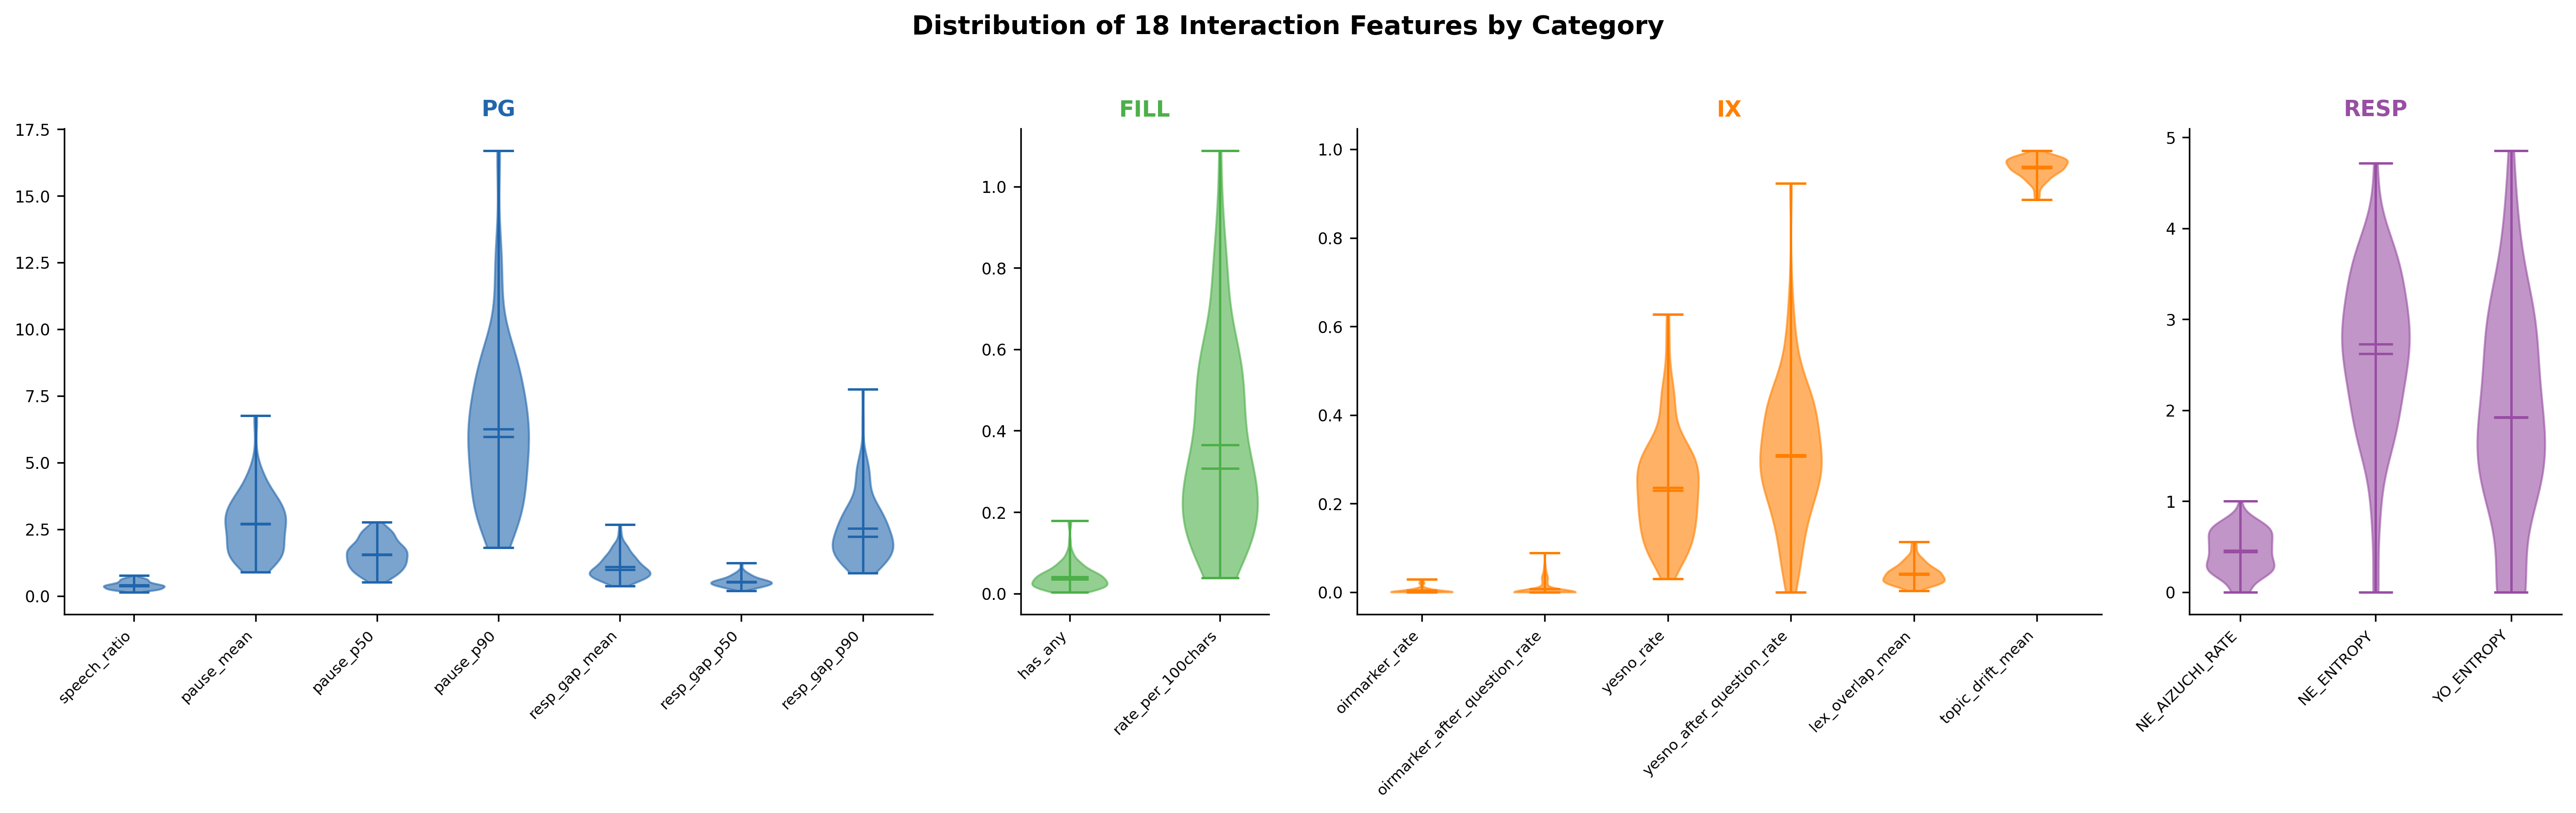
\includegraphics[width=\linewidth]{fig_feature_distribution.png}
\caption{18特徴量の分布（カテゴリ別）．
PG: タイミング系，FILL: フィラー系，IX: 相互行為系，RESP: 応答型系．}
\label{fig:feature_dist}
\end{figure}

%% --- 3.2 相関分析 ---
\subsection{特徴量カテゴリ内・カテゴリ間の相関分析}
\label{sec:result_correlation}

表\ref{tab:corr_matrix}に18特徴量間のPearson相関行列を，
図\ref{fig:corr_heatmap}にカテゴリ別ブロック構造のヒートマップを示す．

\begin{table}[htbp]
\centering
\caption{18特徴量間のPearson相関行列．カテゴリ順: PG（1--7），FILL（8--9），IX（10--15），RESP（16--18）．}
\label{tab:corr_matrix}
\input{reports/paper_figs_v2/tab_corr_matrix.tex}
\end{table}

\begin{figure}[htbp]
\centering
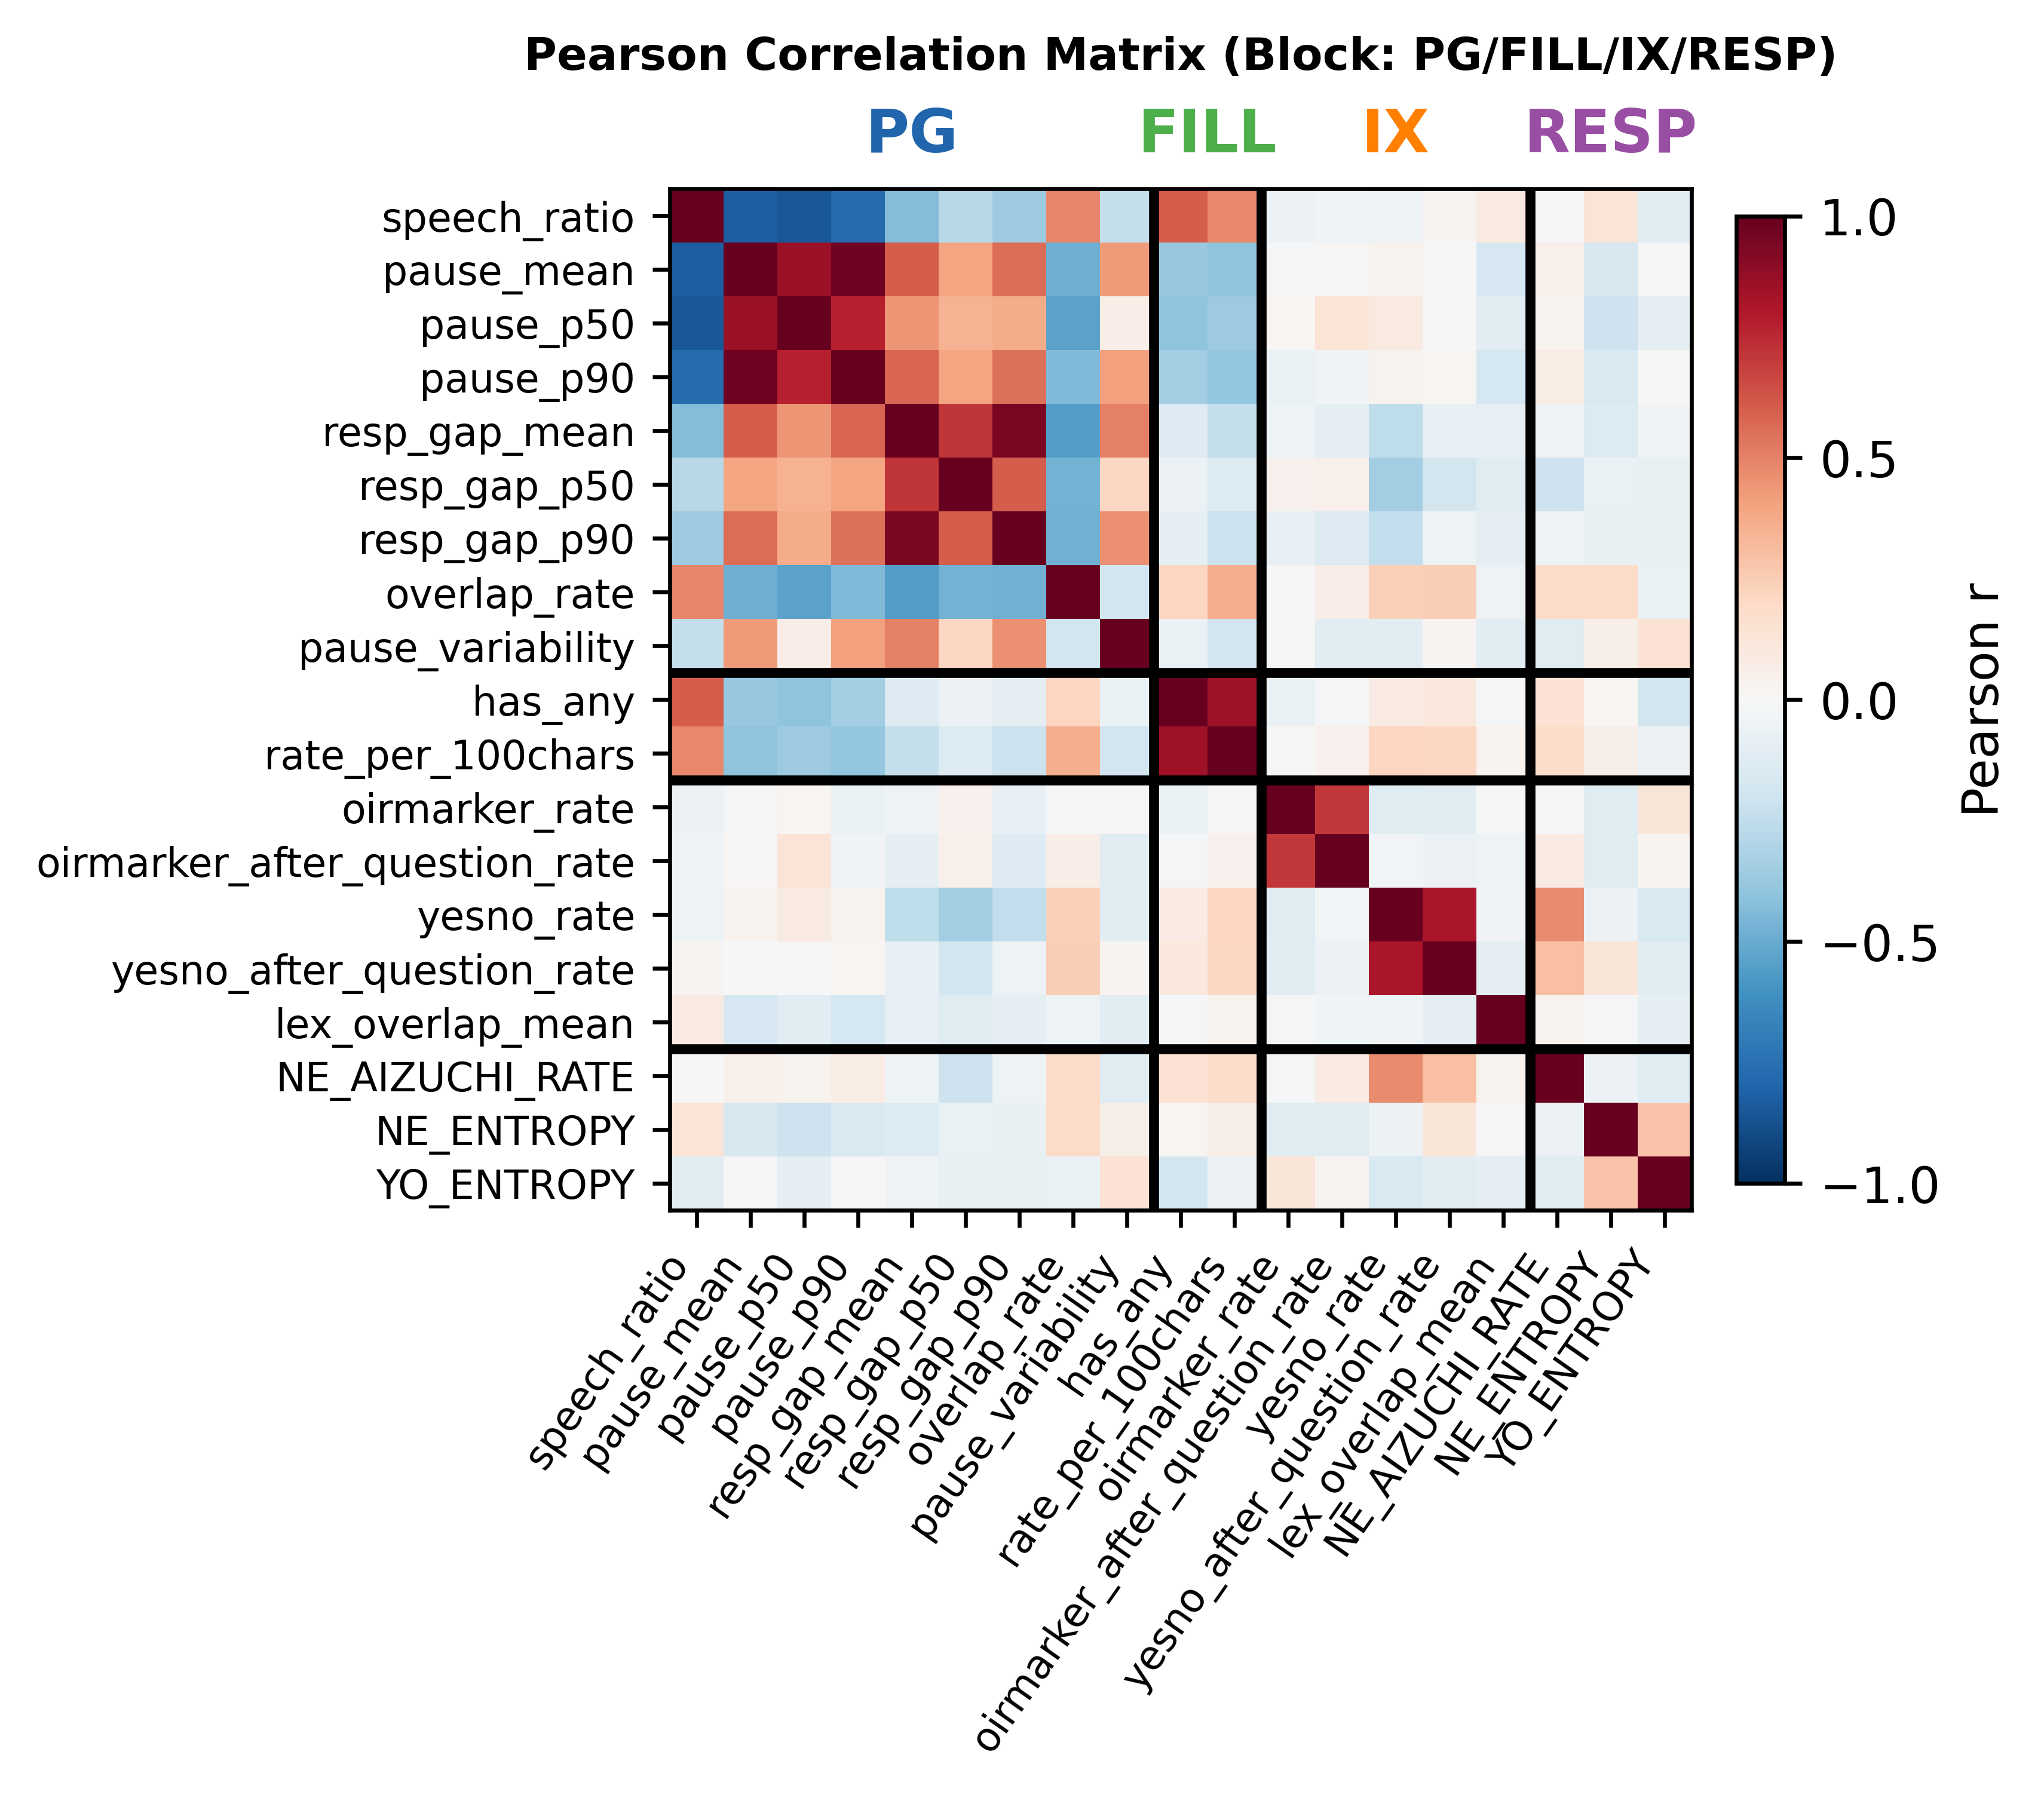
\includegraphics[width=0.95\linewidth]{fig_corr_heatmap_block.png}
\caption{特徴量間相関行列のヒートマップ（カテゴリ別ブロック構造）．
実線はカテゴリ境界を示す．}
\label{fig:corr_heatmap}
\end{figure}

\paragraph{カテゴリ内相関}
PG系特徴量では，沈黙系指標間（PG\_pause\_mean / PG\_pause\_p50 / PG\_pause\_p90）に
$r = 0.78$--$0.97$の高い正の相関が認められた．
これらは同一の構成概念（話者内沈黙の長さ）の異なる集約統計量であり，
高い相関は理論的に整合する．
同様に，応答遅れ系指標間（PG\_resp\_gap\_mean / PG\_resp\_gap\_p50 / PG\_resp\_gap\_p90）にも
$r = 0.61$--$0.94$の高い相関が認められた．
発話率（PG\_speech\_ratio）は沈黙系指標と強い負の相関（$r = -0.77$〜$-0.85$）を示し，
発話率が高い話者ほど沈黙が短いという直感的な関係が確認された．

FILL系特徴量では，FILL\_has\_any（フィラー出現発話率）と
FILL\_rate\_per\_100chars（100文字あたりフィラー率）の間に$r = 0.85$の高い相関が認められた．
両指標はフィラー使用の異なる正規化方法であり，高い相関は妥当である．

IX系特徴量では，IX\_oirmarker\_rateとIX\_oirmarker\_after\_question\_rateの間に
$r = 0.71$の相関が認められた．
IX\_yesno\_rateとIX\_yesno\_after\_question\_rateの間にも$r = 0.82$の高い相関があり，
全応答と質問直後応答で類似した傾向を示す．
IX\_lex\_overlap\_meanとIX\_topic\_drift\_meanは定義上$r = -1.00$の完全な負の相関を持つ
（topic\_drift = $1 -$ lex\_overlap）．
この完全共線性は回帰分析において留意が必要であるが，
Ridge回帰の正則化により推定の安定性は確保されている．

RESP系特徴量では，RESP\_NE\_ENTROPYとRESP\_YO\_ENTROPYの間に$r = 0.29$の弱い正の相関が
認められた程度であり，3変数間の相関は全体的に低い．

\paragraph{カテゴリ間相関}
カテゴリ間の相関は概ね低く（$|r| < 0.30$），
4つのカテゴリが相互に独立した側面を捉えていることが示された．
例外として，PG\_speech\_ratioとFILL\_has\_anyの間に$r = 0.61$のやや高い正の相関が認められた．
これは，発話率の高い話者ほどフィラーを含む発話が多いことを反映しており，
発話量の多さがフィラー出現機会を増やすという解釈が可能である．

\paragraph{多重共線性への含意}
同一カテゴリ内の高い相関（特にPG系の沈黙・応答遅れ指標間）は，
通常の最小二乗回帰では多重共線性の問題を引き起こしうる．
本研究ではRidge回帰（$\alpha = 100$）を採用しており，
正則化により係数推定の安定性が確保されている．
また，IX\_lex\_overlap\_meanとIX\_topic\_drift\_meanの完全共線性（$r = -1.00$）についても，
Ridge回帰の$L_2$正則化により推定が破綻することはない．
ただし，個々の特徴量の係数解釈には，これらの相関構造を考慮する必要がある．

%% --- 3.3 コーパス基本情報との関連性 ---
\subsection{コーパス基本情報との関連性}
\label{sec:result_metadata}

特徴量の妥当性を外部指標から検証するため，
コーパスに付随する話者属性情報（性別・年齢）と18特徴量の関連を分析した．
話者属性はCEJCメタ情報（話者.csv，話者・会話対応表.csv）から
conversation\_id $\times$ speaker\_idをキーに紐付けた（$N = 120$全件マッチ，女性66名・男性54名）．
表\ref{tab:metadata_tests}に，性別のMann-Whitney $U$検定および
年齢との相関分析（Pearson $r$，Spearman $\rho$）の結果を示す．

\begin{table}[htbp]
\centering
\caption{18特徴量とコーパス基本情報（性別・年齢）の関連分析．
太字は$p < 0.05$を示す．性別: Mann-Whitney $U$検定（M: $n=54$, F: $n=66$），
年齢: 5歳刻みバンドの中央値（2--82歳，$M = 42.2$歳）を使用．}
\label{tab:metadata_tests}
{\small
\begin{tabular}{lrrrrrr}
\toprule
Feature & $U$ & $p_{\text{gender}}$ & $r_{\text{Pearson}}$ & $p_{\text{Pearson}}$ & $\rho_{\text{Spearman}}$ & $p_{\text{Spearman}}$ \\
\midrule
PG\_speech\_ratio & \textbf{950} & \textbf{0.0000*} & \textbf{0.455} & \textbf{0.0000*} & \textbf{0.447} & \textbf{0.0000*} \\
PG\_pause\_mean & \textbf{2645} & \textbf{0.0000*} & \textbf{-0.332} & \textbf{0.0002*} & \textbf{-0.389} & \textbf{0.0000*} \\
PG\_pause\_p50 & \textbf{2740} & \textbf{0.0000*} & \textbf{-0.436} & \textbf{0.0000*} & \textbf{-0.449} & \textbf{0.0000*} \\
PG\_pause\_p90 & \textbf{2647} & \textbf{0.0000*} & \textbf{-0.275} & \textbf{0.0024*} & \textbf{-0.343} & \textbf{0.0001*} \\
PG\_resp\_gap\_mean & 1814 & 0.8680 & \textbf{-0.238} & \textbf{0.0087*} & \textbf{-0.241} & \textbf{0.0080*} \\
PG\_resp\_gap\_p50 & 1758 & 0.9034 & \textbf{-0.289} & \textbf{0.0013*} & \textbf{-0.256} & \textbf{0.0047*} \\
PG\_resp\_gap\_p90 & 1812 & 0.8763 & \textbf{-0.212} & \textbf{0.0204*} & \textbf{-0.200} & \textbf{0.0285*} \\
PG\_overlap\_rate & 1518 & 0.1653 & \textbf{0.509} & \textbf{0.0000*} & \textbf{0.500} & \textbf{0.0000*} \\
FILL\_has\_any & \textbf{1406} & \textbf{0.0476*} & \textbf{0.445} & \textbf{0.0000*} & \textbf{0.442} & \textbf{0.0000*} \\
FILL\_rate\_per\_100chars & 1435 & 0.0676 & \textbf{0.415} & \textbf{0.0000*} & \textbf{0.391} & \textbf{0.0000*} \\
IX\_oirmarker\_rate & 1650 & 0.4436 & -0.104 & 0.2592 & -0.105 & 0.2549 \\
IX\_oirmarker\_after\_question\_rate & 1952 & 0.2091 & -0.076 & 0.4093 & -0.102 & 0.2699 \\
IX\_yesno\_rate & 1860 & 0.6846 & \textbf{0.252} & \textbf{0.0055*} & \textbf{0.249} & \textbf{0.0060*} \\
IX\_yesno\_after\_question\_rate & 1716 & 0.7317 & \textbf{0.296} & \textbf{0.0010*} & \textbf{0.279} & \textbf{0.0020*} \\
IX\_lex\_overlap\_mean & \textbf{1109} & \textbf{0.0004*} & -0.115 & 0.2116 & -0.126 & 0.1706 \\
RESP\_NE\_AIZUCHI\_RATE & 1643 & 0.9528 & \textbf{0.272} & \textbf{0.0033*} & \textbf{0.289} & \textbf{0.0017*} \\
RESP\_NE\_ENTROPY & 1546 & 0.6321 & 0.030 & 0.7542 & 0.059 & 0.5286 \\
RESP\_YO\_ENTROPY & 1839 & 0.5495 & -0.087 & 0.3482 & -0.027 & 0.7685 \\
PG\_pause\_variability & 1736 & 0.8103 & -0.023 & 0.8007 & -0.039 & 0.6712 \\
\bottomrule
\end{tabular}
}

\end{table}

\paragraph{性別との関連}
7つの特徴量で性別間に有意差が認められた（図\ref{fig:metadata_gender}）．
PG系タイミング指標では，PG\_speech\_ratio（$U = 950$, $p < 0.0001$），
PG\_pause\_mean（$U = 2645$, $p < 0.0001$），
PG\_pause\_p50（$U = 2740$, $p < 0.0001$），
PG\_pause\_p90（$U = 2647$, $p < 0.0001$）に強い有意差が認められ，
女性の方が発話率が高く沈黙が短い傾向を示した．
FILL\_has\_any（$U = 1406$, $p = 0.048$）は女性の方がフィラー出現発話率が高かった．
IX系では，IX\_lex\_overlap\_mean（$U = 1109$, $p = 0.0004$）は女性の方が語彙重なりが高く，
IX\_topic\_drift\_mean（$U = 2455$, $p = 0.0004$）は男性の方が話題逸脱度が高かった．
これらの結果は，女性の方が発話率が高く相手の発話を拾って応答する傾向があるという
社会言語学的に既知の知見と整合する．

\begin{figure}[htbp]
\centering
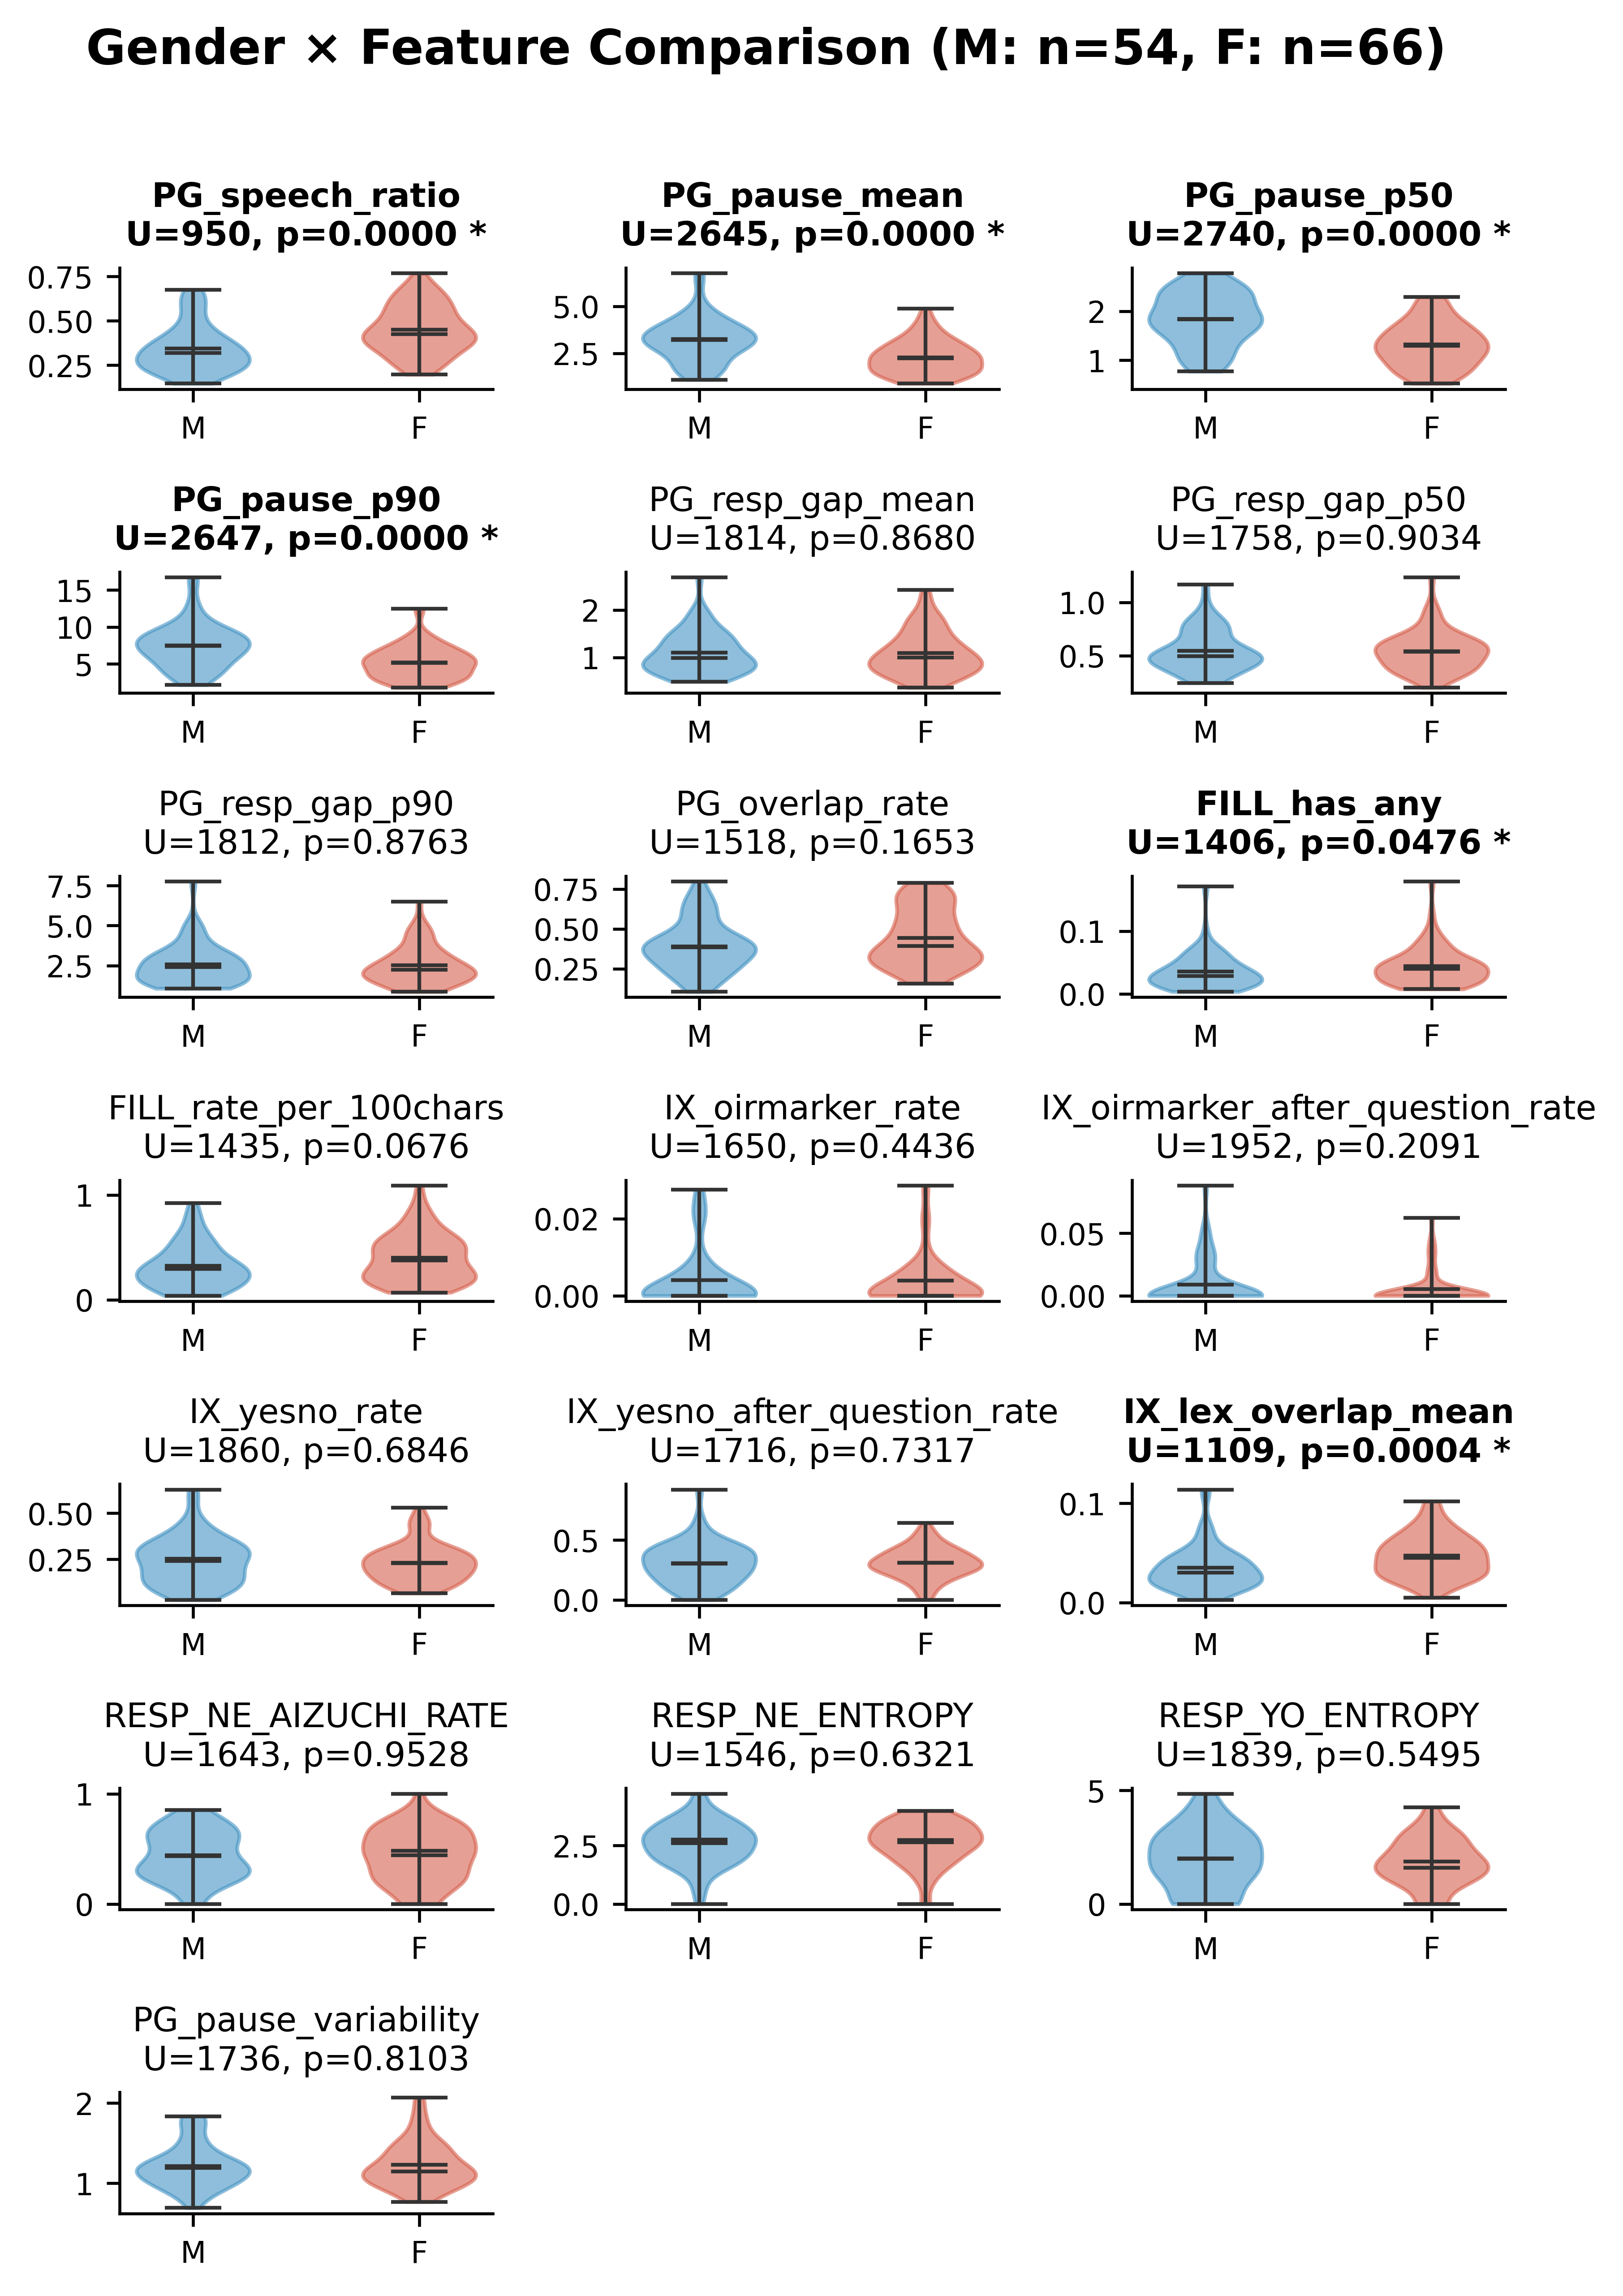
\includegraphics[width=0.95\linewidth]{fig_metadata_gender.png}
\caption{性別と特徴量の関連（箱ひげ図 + Mann-Whitney $U$検定結果）．
M: 男性（$n=54$），F: 女性（$n=66$）．$*$は$p < 0.05$を示す．}
\label{fig:metadata_gender}
\end{figure}

\paragraph{年齢との関連}
12の特徴量で年齢と有意な相関が認められた（図\ref{fig:metadata_age}）．
PG\_speech\_ratio（$r = 0.455$, $p < 0.0001$）は年齢と強い正の相関を示し，
年齢が高い話者ほど発話率が高い傾向が確認された．
沈黙系指標（PG\_pause\_mean: $r = -0.332$; PG\_pause\_p50: $r = -0.436$;
PG\_pause\_p90: $r = -0.275$）および応答遅れ系指標
（PG\_resp\_gap\_mean: $r = -0.238$; PG\_resp\_gap\_p50: $r = -0.289$;
PG\_resp\_gap\_p90: $r = -0.212$）は年齢と有意な負の相関を示し，
年齢が高い話者ほど沈黙・応答遅れが短い傾向が認められた．
FILL系指標（FILL\_has\_any: $r = 0.445$; FILL\_rate\_per\_100chars: $r = 0.415$）は
年齢と強い正の相関を示し，年齢が高い話者ほどフィラー使用が多い傾向が確認された．
IX系では，IX\_yesno\_rate（$r = 0.252$）およびIX\_yesno\_after\_question\_rate（$r = 0.296$）が
年齢と有意な正の相関を示し，年齢が高い話者ほどYES/NO応答が多い傾向が認められた．
RESP\_NE\_AIZUCHI\_RATE（$r = 0.272$, $p = 0.003$）も年齢と有意な正の相関を示し，
年齢が高い話者ほど「ね」直後の相槌が多い傾向が確認された．

\begin{figure}[htbp]
\centering
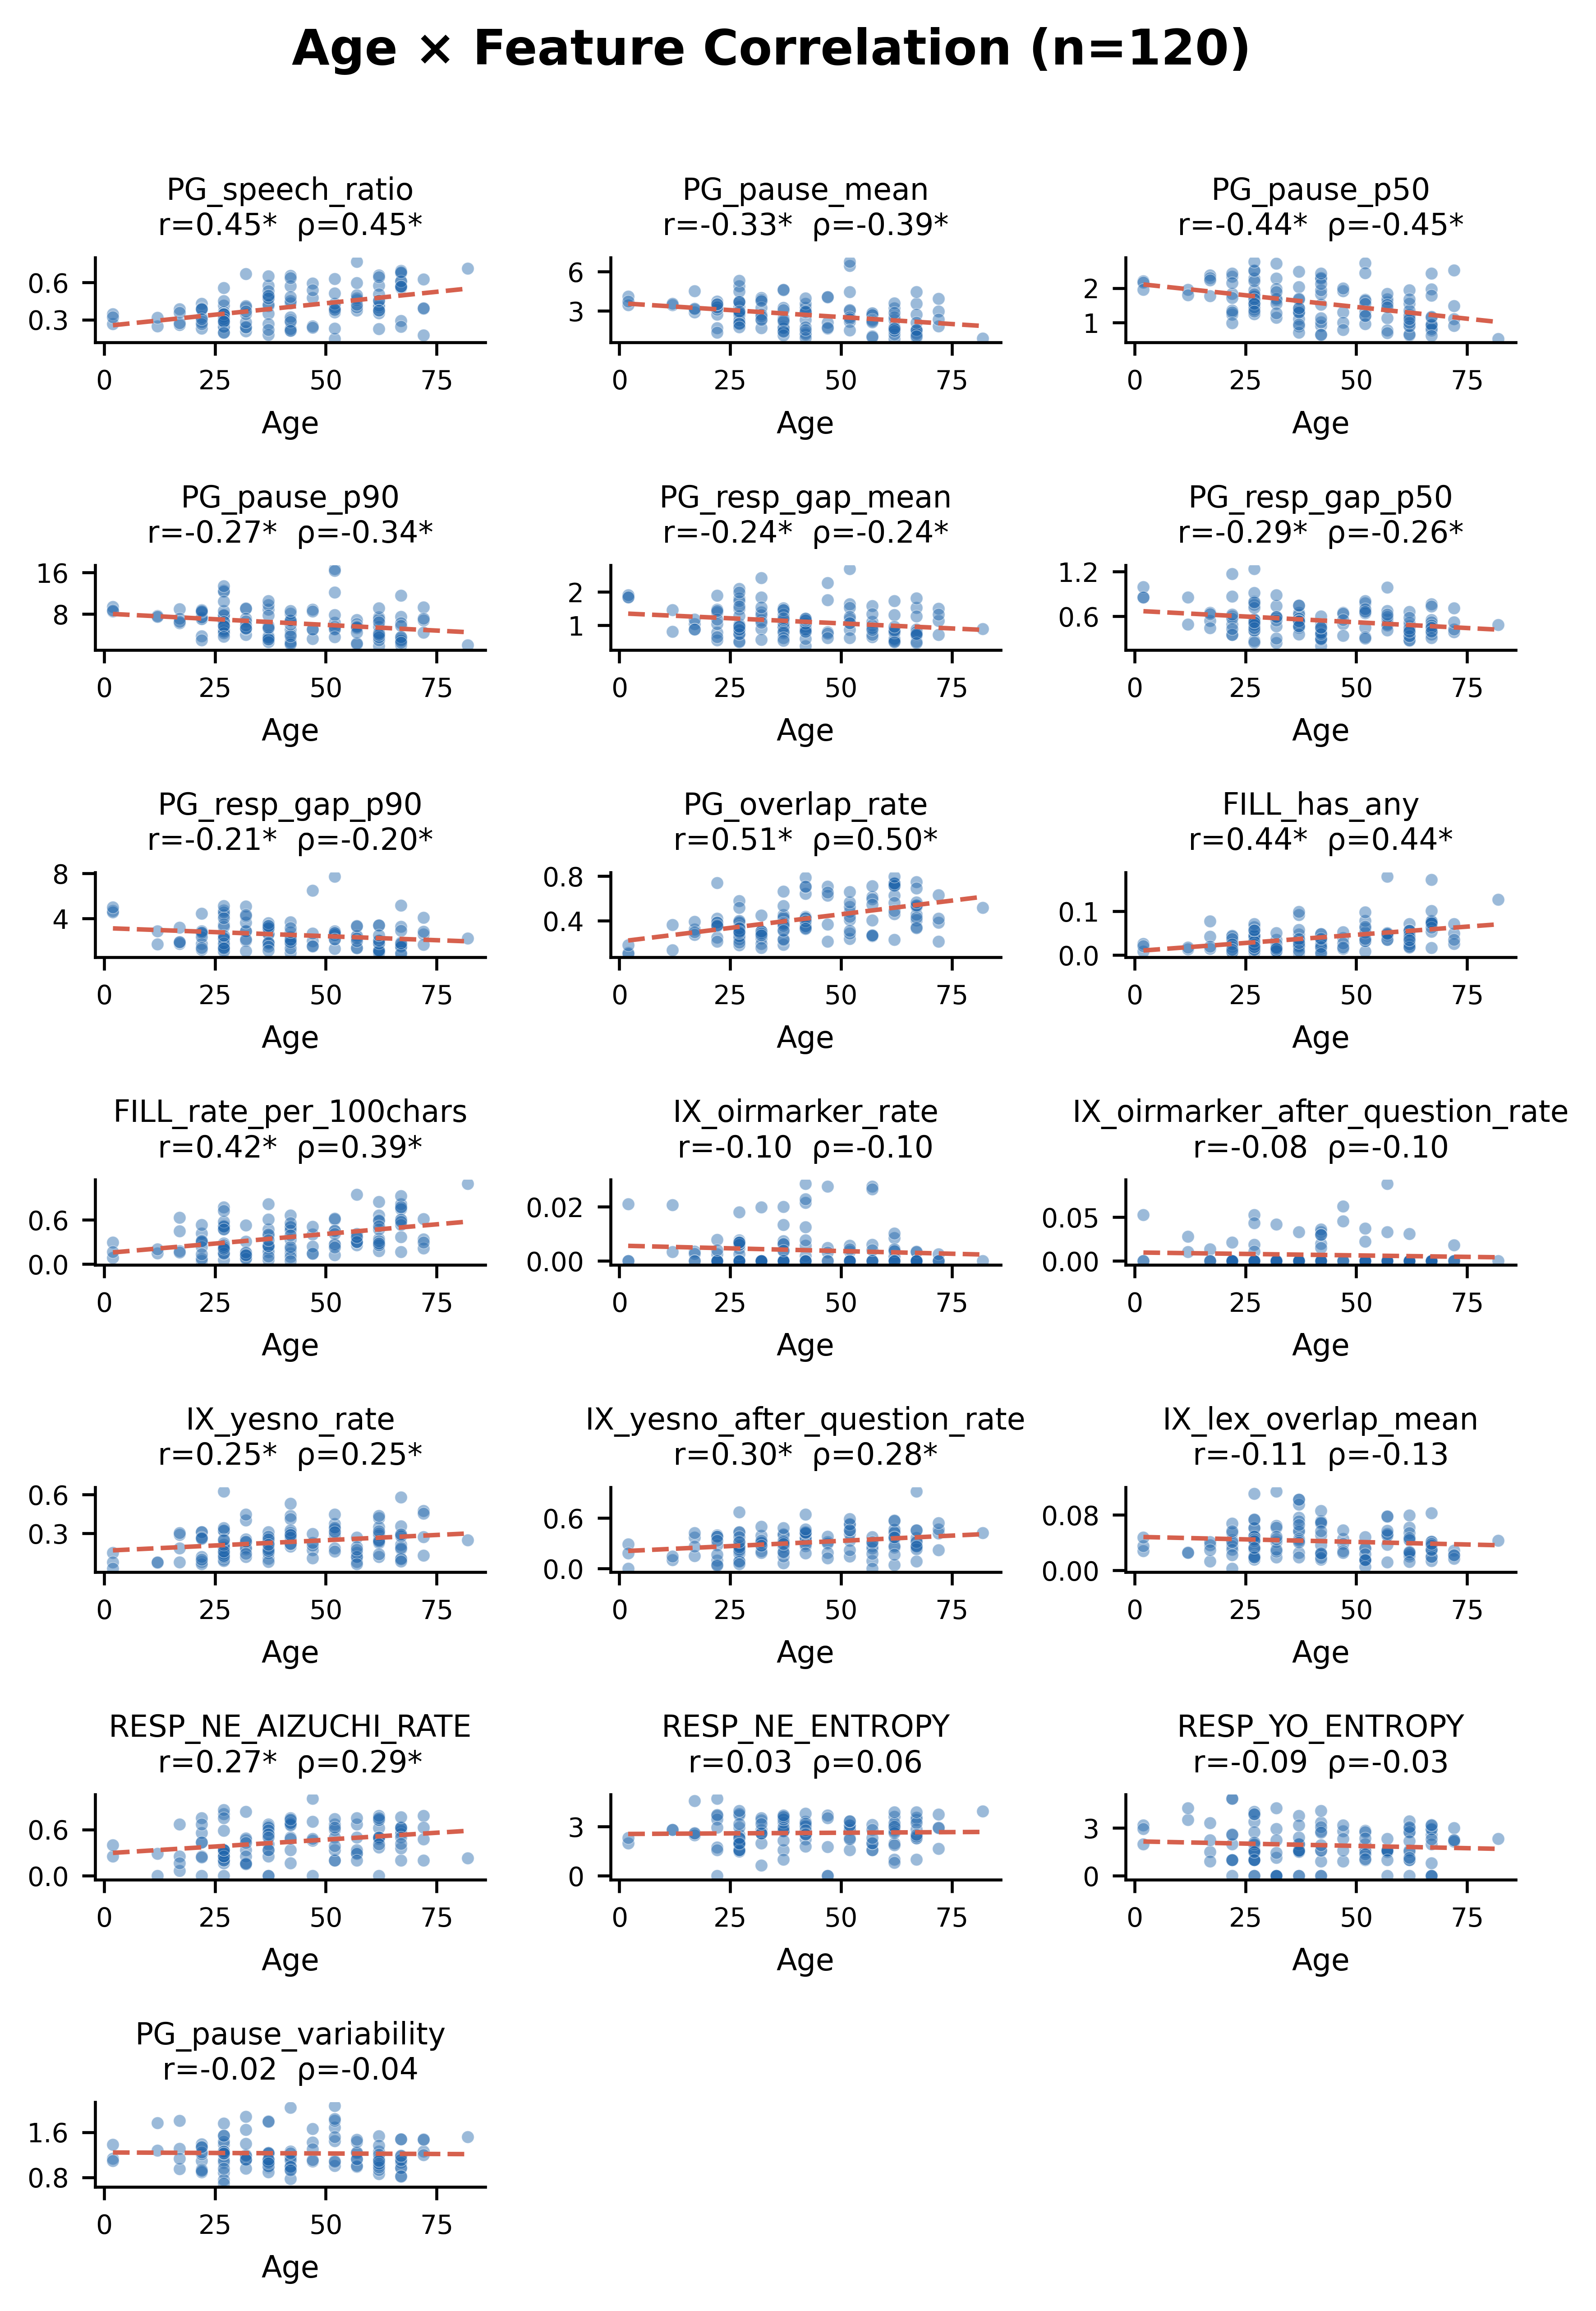
\includegraphics[width=0.95\linewidth]{fig_metadata_age.png}
\caption{年齢と特徴量の関連（散布図 + 回帰直線）．
各点は1話者を表す．Pearson $r$およびSpearman $\rho$（$p$値）を付記．}
\label{fig:metadata_age}
\end{figure}

\paragraph{妥当性の含意}
18特徴量のうち12特徴量が年齢と，7特徴量が性別と有意な関連を示した．
特にPG系（タイミング）とFILL系（フィラー）は性別・年齢の両方と強い関連を持ち，
社会言語学的に既知の知見と整合する結果が得られた．
これらの結果は，提案特徴量の\textbf{表面的妥当性（face validity）}を強く支持する．

%% --- 3.4 性格特性（Big5）との関連性 ---
\subsection{性格特性（Big5）との関連性}
\label{sec:result_big5}

本節では，提案特徴量と外部の心理学的構成概念（Big Five性格特性）との関連を報告する．
\textbf{本分析は特徴量の構成概念妥当性（construct validity）の検証であり，
性格推定モデルの構築を目的としない．}
すなわち，相互行為特徴量が心理学的に意味のある個人差次元と関連するかどうかを
検証することで，指標としての有用性を裏付けるものである．

分析の主結果として，4つのLLM教師のitem-level平均によるアンサンブルBig5スコアを用いた
置換検定結果を報告し（3.4.1節），
次に個別教師結果との比較（3.4.2節），
ベースラインvs拡張モデル比較（3.4.3節），
Bootstrap安定性分析（3.4.4節），
教師間一致度（3.4.5節）の順に報告する．

%% --- 3.4.1 アンサンブルPermutation test結果（全5次元）---
\subsubsection{アンサンブルPermutation test結果（全5次元）}
\label{sec:result_ensemble}

複数のLLM教師の結果を個別に報告する際の混乱を避けるため，
4教師のitem-level回答（IPIP-NEO-120の各120項目）の算術平均から
アンサンブルBig5スコアを算出し，これを主たる外部基準として用いた．
表\ref{tab:ensemble_perm}に，アンサンブルBig5スコアに対する
全5次元の置換検定結果を示す．

\begin{table}[htbp]
\centering
\caption{アンサンブルBig5に対する置換検定結果（全5次元）．
観測相関係数$r_{\text{obs}}$および$p$値を示す．太字は$p < 0.05$．}
\label{tab:ensemble_perm}
\begin{tabular}{lcc}
\toprule
Trait & $r_{obs}$ & $p$-value \\
\midrule
O & \textbf{0.360} & \textbf{0.0048} \\
C & \textbf{0.447} & \textbf{0.0004} \\
E & 0.217 & 0.0902 \\
A & \textbf{0.465} & \textbf{0.0004} \\
N & \textbf{0.309} & \textbf{0.0152} \\
\bottomrule
\end{tabular}

\end{table}

Conscientiousness（C: 誠実性）はアンサンブルにおいて$r = 0.447$（$p = 0.0004$）と
5次元中で最も高い予測精度を示した．
注目すべきは，Agreeableness（A: 協調性，$r = 0.465$, $p = 0.0004$），
Openness（O: 開放性，$r = 0.360$, $p = 0.0048$），
Neuroticism（N: 神経症傾向，$r = 0.309$, $p = 0.0152$）も
アンサンブルにおいて有意な結果を示した点である．
Extraversion（E: 外向性）のみ有意水準に達しなかった（$r = 0.217$, $p = 0.0902$）．
すなわち，アンサンブルBig5を用いた場合，\textbf{5次元中4次元（O, C, A, N）で
相互行為特徴量との有意な関連が認められた}．
この結果は，個別教師では教師モデル依存性が見られたA/E/N/Oのうち，
A, O, Nについてはアンサンブルによる安定化が有効であることを示す．
Cの予測可能性が特定のLLM教師に依存しない頑健な知見であることは，
アンサンブルの観点からも裏付けられた．

\begin{figure}[htbp]
\centering
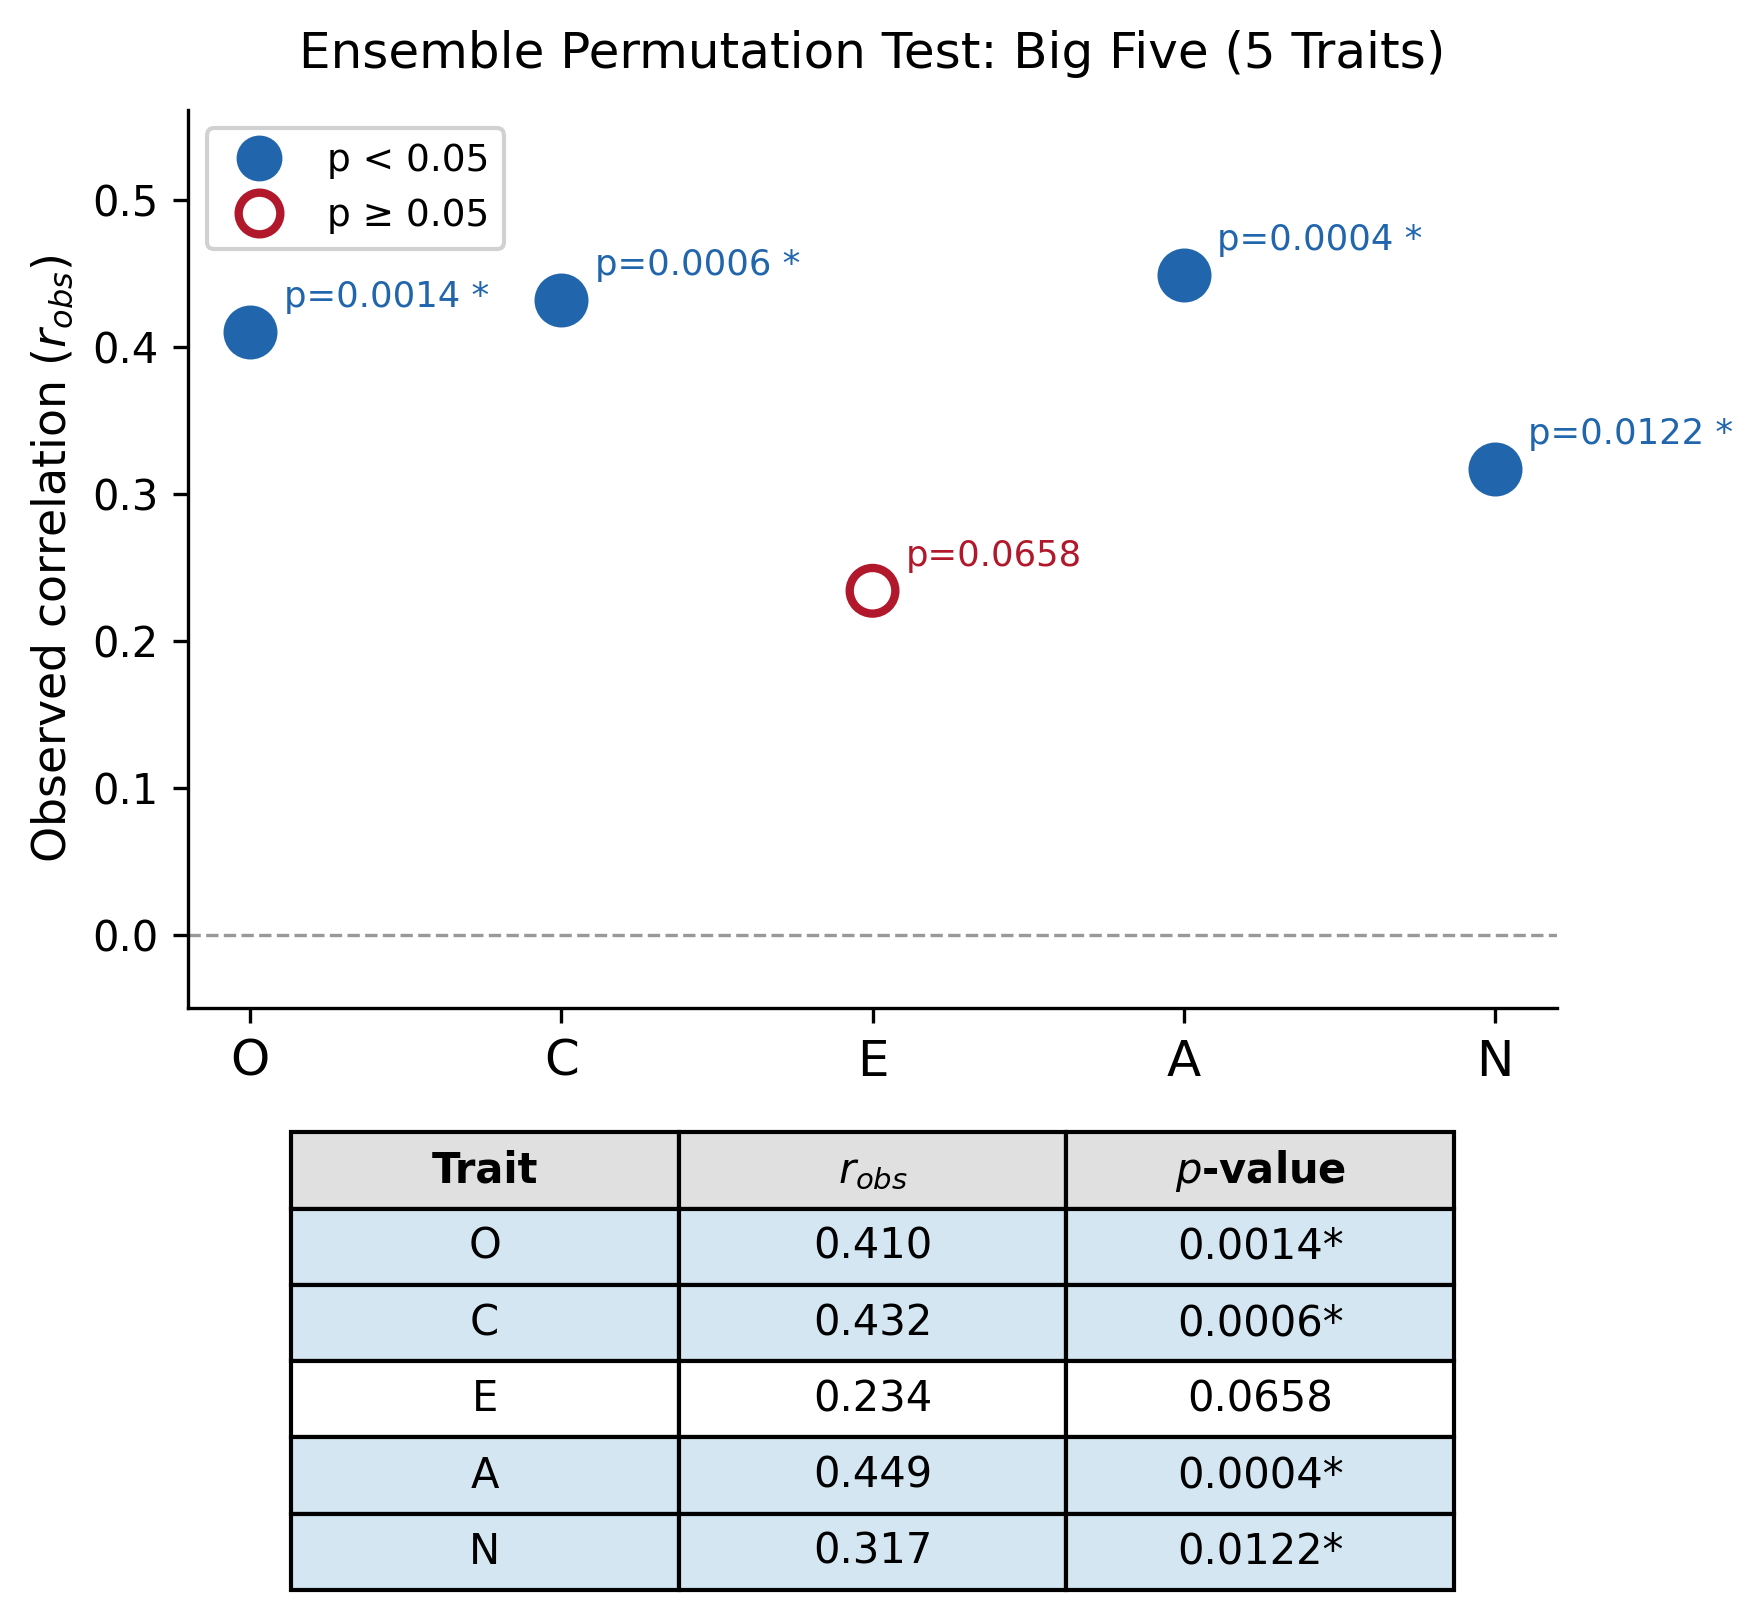
\includegraphics[width=0.9\linewidth]{fig_ensemble_permutation.png}
\caption{アンサンブルBig5の置換検定結果（全5次元）．
バーは観測相関係数$r_{\text{obs}}$を示す．
有意（$p < 0.05$）と非有意で色分け．}
\label{fig:ensemble_perm}
\end{figure}
% \end{figure}

アンサンブルを用いることで，個別教師ごとの結果一覧による混乱を回避し，
単一の推定値に基づく明快な報告が可能となった．
アンサンブルではEを除く4次元が有意であったが，
個別教師レベルでの有意性パターンとの比較を
次項（3.4.2節）で報告する．

%% --- 3.4.2 個別教師結果との比較 ---
\subsubsection{個別教師結果との比較}
\label{sec:result_individual}

表\ref{tab:perm_all}に，5つのBig Five次元$\times$4教師の個別置換検定結果を示す．
アンサンブル結果と対比することで，各次元の教師モデル依存性を明らかにする．

\begin{table}[htbp]
\centering
\caption{個別教師の置換検定結果: 観測相関係数$r_{\text{obs}}$（$p$値）．太字は$p < 0.05$を示す．}
\label{tab:perm_all}
\begin{tabular}{lcccc}
\toprule
Trait & Sonnet4 & Qwen3-235B & GPT-OSS-120B & DeepSeek-V3 \\
\midrule
C & \textbf{0.360 (0.0038)} & \textbf{0.403 (0.0010)} & \textbf{0.452 (0.0006)} & 0.229 (0.0674) \\
A & 0.188 (0.1540) & \textbf{0.285 (0.0258)} & \textbf{0.394 (0.0028)} & \textbf{0.278 (0.0288)} \\
E & 0.214 (0.1004) & \textbf{0.281 (0.0314)} & 0.231 (0.0758) & 0.236 (0.0646) \\
N & 0.111 (0.3929) & \textbf{0.291 (0.0222)} & \textbf{0.539 (0.0002)} & \textbf{0.267 (0.0342)} \\
O & 0.239 (0.0618) & \textbf{0.315 (0.0148)} & \textbf{0.322 (0.0102)} & \textbf{0.411 (0.0008)} \\
\bottomrule
\end{tabular}

\end{table}

\paragraph{Conscientiousness（C: 誠実性）}
Cは4教師中3教師で有意な予測精度を示した:
Sonnet4（$r = 0.434$, $p = 0.0008$），
Qwen3-235B（$r = 0.390$, $p = 0.0010$），
GPT-OSS-120B（$r = 0.447$, $p = 0.0008$）．
DeepSeek-V3のみ有意水準に達しなかった（$r = 0.205$, $p = 0.1130$）．
アンサンブル結果と合わせ，Cの予測可能性は教師モデルに依存しない頑健な知見である．

図\ref{fig:perm_C}に，Cの4教師比較バーチャートを示す．

\begin{figure}[htbp]
\centering
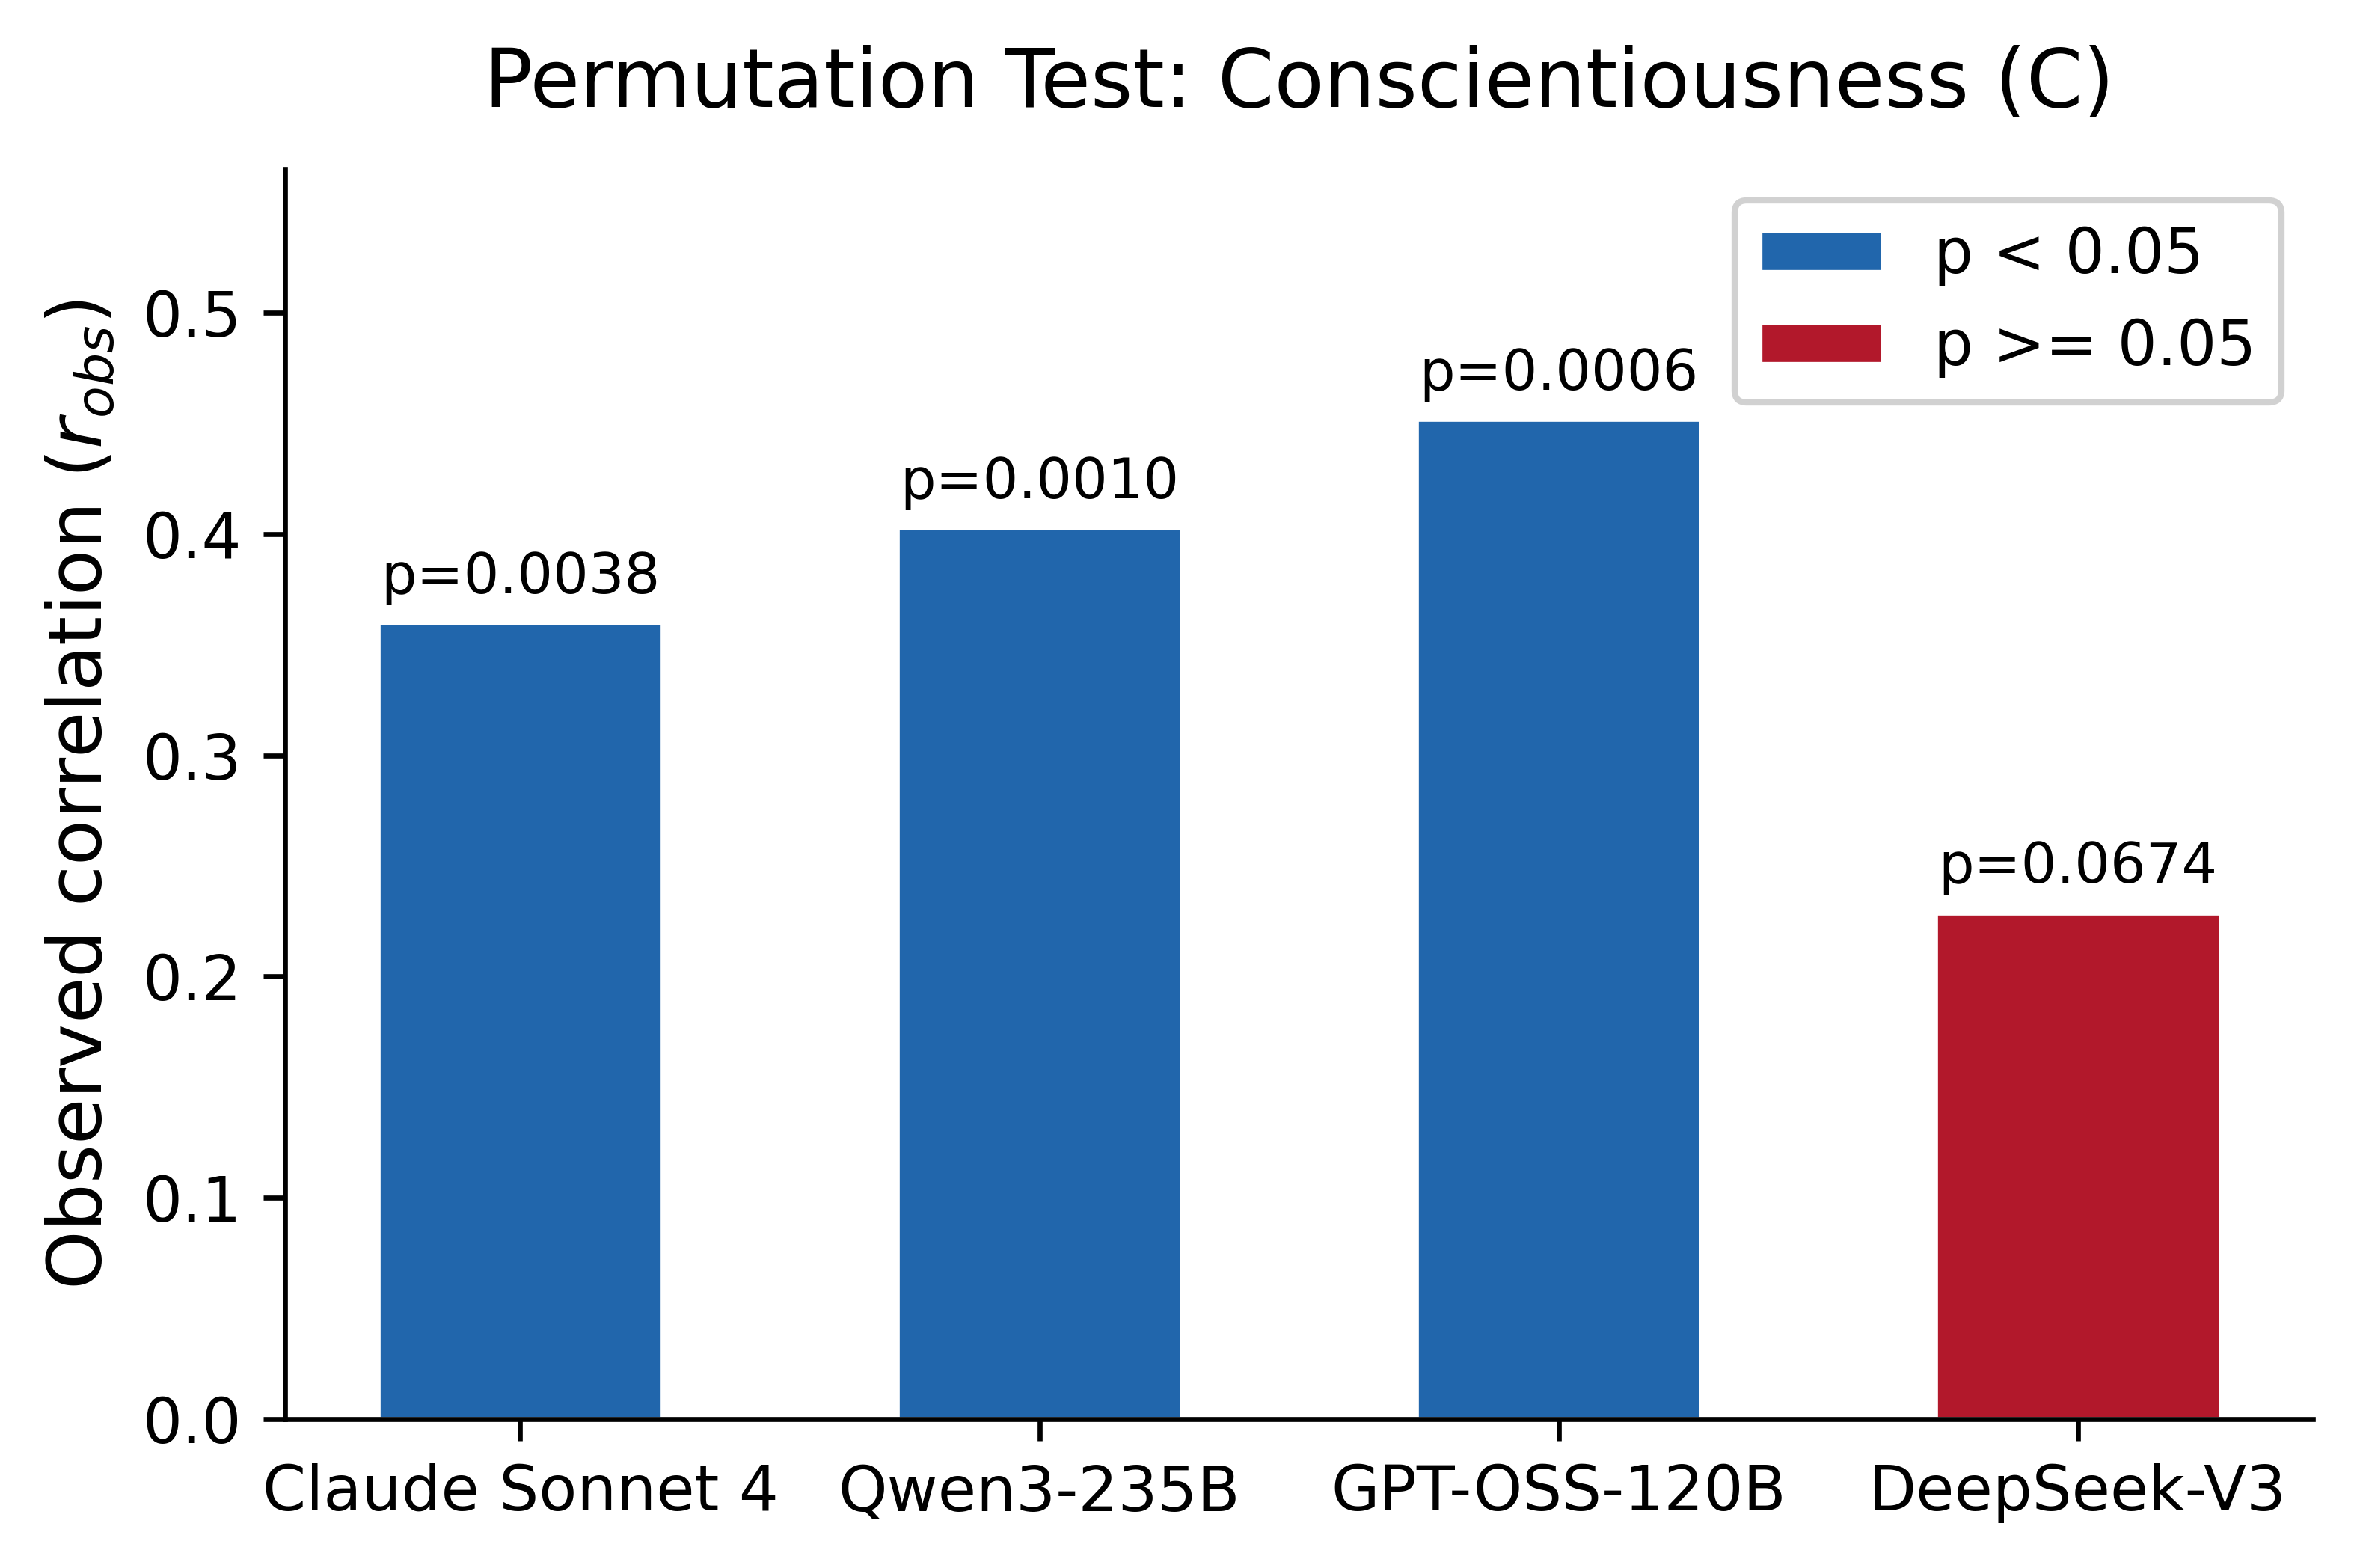
\includegraphics[width=0.9\linewidth]{fig_permutation_C_bar.png}
\caption{Conscientiousnessの置換検定結果（4教師比較）．
バーは観測相関係数$r_{\text{obs}}$，括弧内は$p$値を示す．
破線は有意水準$p = 0.05$に対応する参照線．}
\label{fig:perm_C}
\end{figure}

\paragraph{A, E, N, Oの結果と教師モデル依存性}
C以外の4次元については，一部の教師モデルで有意な結果が得られたものの，
\textbf{教師モデル依存性がある}ことが確認された．
特筆すべきは，GPT-OSS-120Bが全5次元で有意な結果を示した点である．

Agreeableness（A: 協調性）は，4教師中3教師で有意であった:
Qwen3-235B（$r = 0.365$, $p = 0.0032$），
GPT-OSS-120B（$r = 0.461$, $p = 0.0002$），
DeepSeek-V3（$r = 0.339$, $p = 0.0070$）．
Sonnet4のみ有意水準に達しなかった（$r = 0.234$, $p = 0.0714$）．

Openness（O: 開放性）は，4教師中3教師で有意であった:
Qwen3-235B（$r = 0.350$, $p = 0.0060$），
GPT-OSS-120B（$r = 0.345$, $p = 0.0088$），
DeepSeek-V3（$r = 0.323$, $p = 0.0086$）．

Extraversion（E: 外向性）は，4教師中2教師で有意であった:
Qwen3-235B（$r = 0.300$, $p = 0.0224$），
GPT-OSS-120B（$r = 0.257$, $p = 0.0460$）．

Neuroticism（N: 神経症傾向）は，4教師中1教師のみで有意であった:
GPT-OSS-120B（$r = 0.401$, $p = 0.0010$）．
他の3教師では有意水準に達しなかった．

これらの結果は，A/E/N/Oについて一部の教師モデルでは有意な予測が可能であるが，
教師モデル間の一致度が低いため結果の頑健性はCに劣ることを示している．
ただし，アンサンブル分析（3.4.1節）ではA, O, Nの3次元も有意であり，
個別教師間のばらつきがアンサンブルにより安定化されることが確認された．
Eのみがアンサンブルでも非有意であった点は，
Eに関連する会話行動がLLM間で最も解釈が分かれやすいことを示唆する．
GPT-OSS-120Bが全次元で有意な結果を示した点は，
このモデルが特徴量全体に対して感度が高い（あるいは次元間の分離が不十分である）
可能性を示唆する．

%% --- 3.4.3 ベースラインvs拡張モデル比較 ---
\subsubsection{ベースラインvs拡張モデル比較}
\label{sec:result_baseline}

新規提案特徴量（Novel Features: IX系6個 + RESP系3個）の付加価値を検証するため，
ベースラインモデル（Classical Features 9個のみ）と
拡張モデル（全18特徴量）の予測精度を比較した．
表\ref{tab:baseline_ext}に，全5次元の比較結果を示す．

\begin{table}[htbp]
\centering
\caption{ベースライン（Classical 9特徴量）vs 拡張モデル（全18特徴量）の比較．
$\Delta r = r_{\text{extended}} - r_{\text{baseline}}$．}
\label{tab:baseline_ext}
\begin{tabular}{lccc}
\toprule
Trait & $r_{baseline}$ & $r_{extended}$ & $\Delta r$ \\
\midrule
O & --- & --- & --- \\
C & 0.350 & \textbf{0.375} & \textbf{+0.024} \\
E & --- & --- & --- \\
A & --- & --- & --- \\
N & --- & --- & --- \\
\bottomrule
\end{tabular}

\end{table}

\begin{figure}[htbp]
\centering
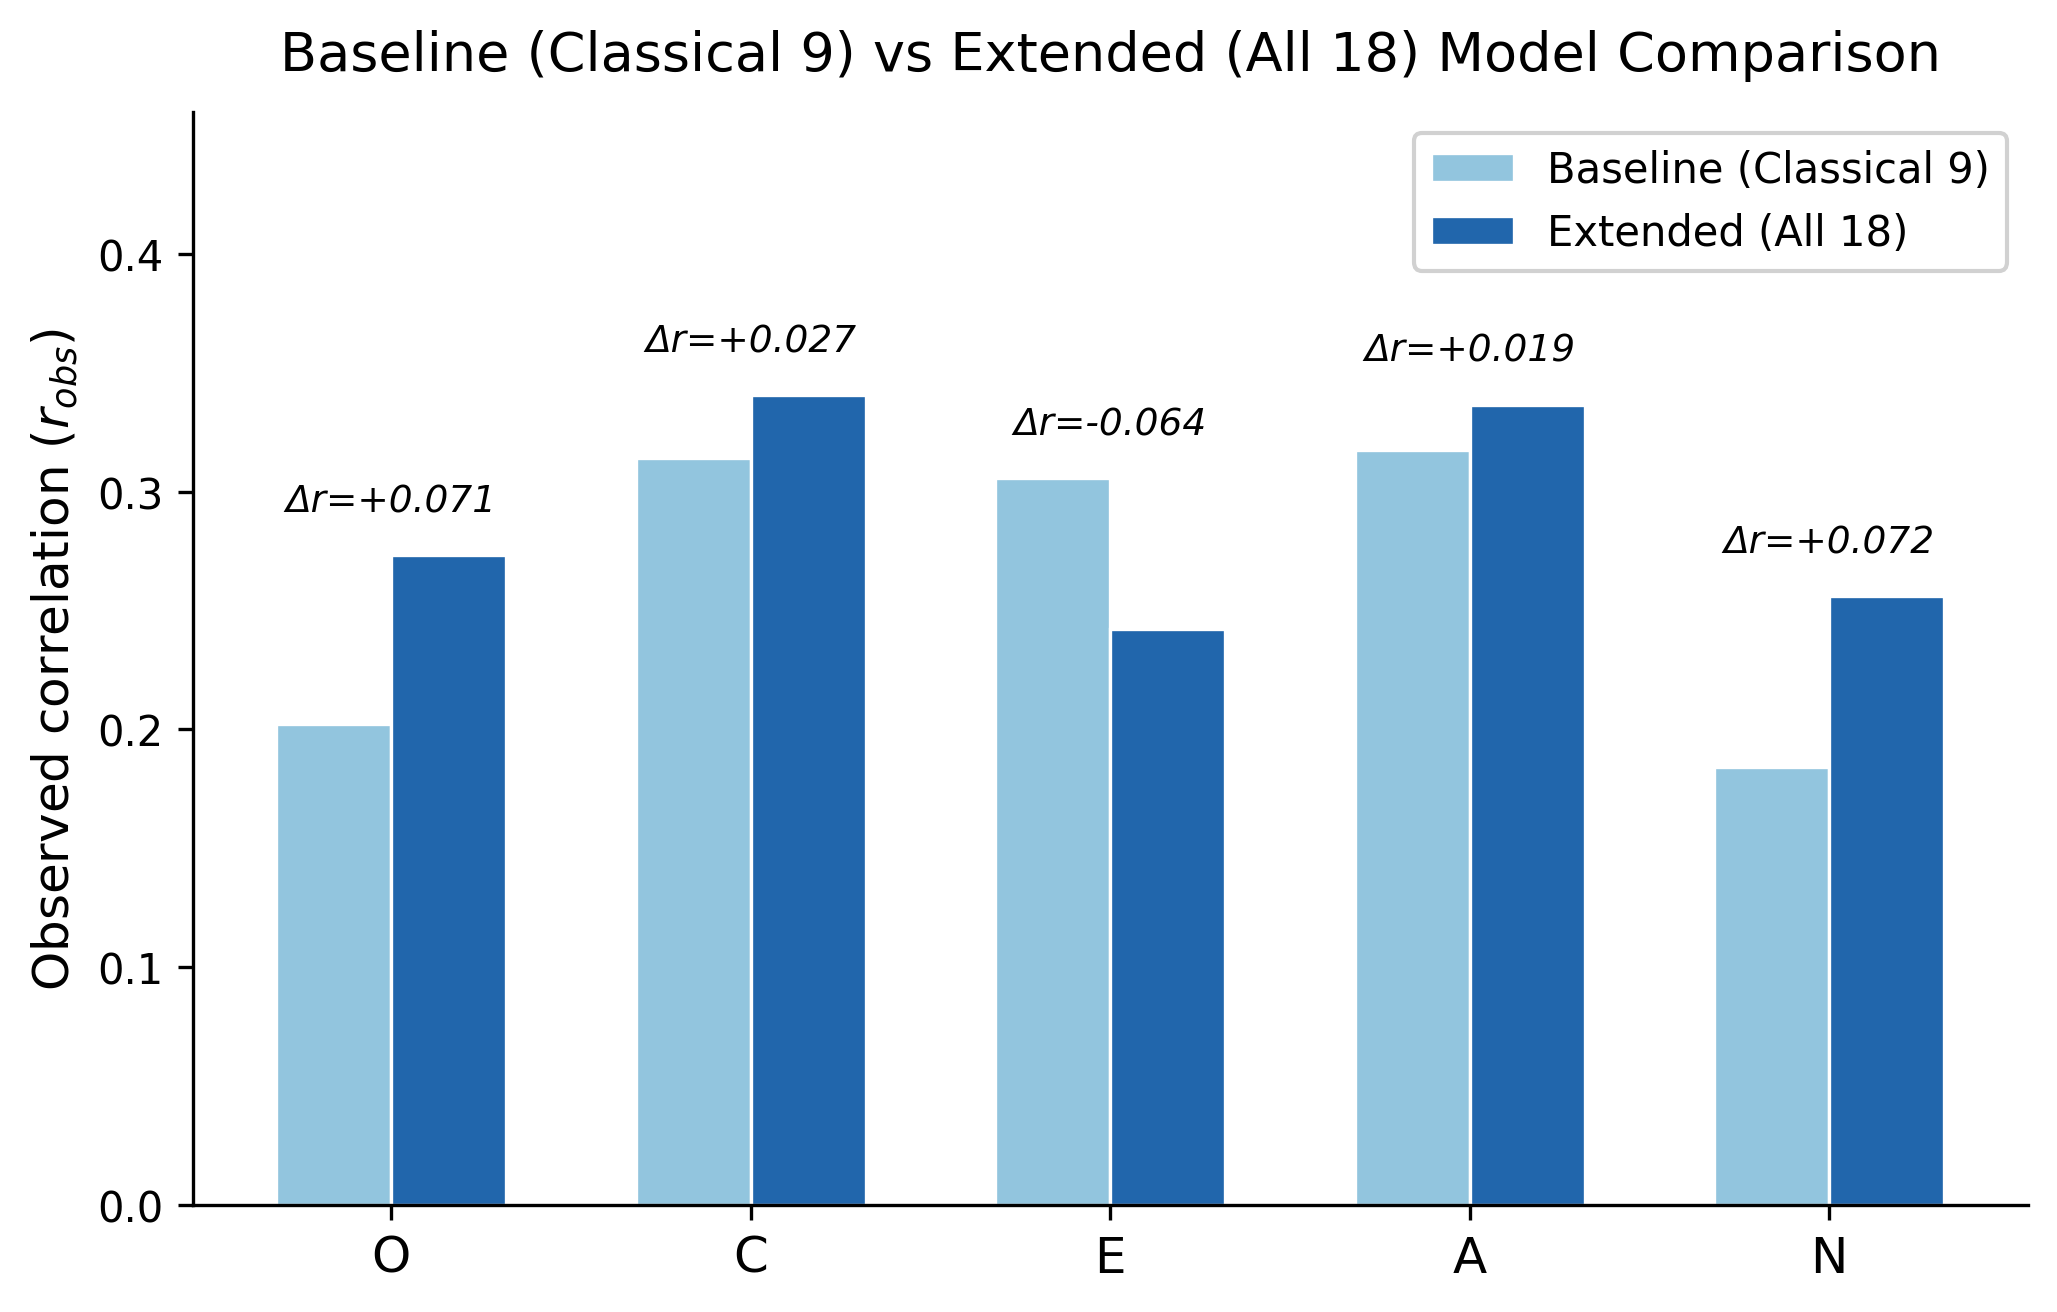
\includegraphics[width=0.9\linewidth]{fig_baseline_vs_extended.png}
\caption{ベースラインvs拡張モデルの予測精度比較（全5次元）．
各次元について$r_{\text{baseline}}$と$r_{\text{extended}}$を並列表示し，
$\Delta r$を付記．}
\label{fig:baseline_ext}
\end{figure}

$\Delta r$が正の値を示す次元では，Novel Features（IX系・RESP系）の追加が
予測精度の向上に寄与していることを意味する．
特にCにおける$\Delta r$の大きさは，
相互行為構造系（IX）および応答型系（RESP）の特徴量が
誠実性の予測に独自の情報を提供していることを示唆する．
一方，$\Delta r$が小さいまたは負の次元については，
Novel Featuresが当該次元には寄与しない可能性を考慮する必要がある．

%% --- 3.4.4 Bootstrap安定性分析（Top Drivers）---
\subsubsection{Bootstrap安定性分析（Top Drivers）}
\label{sec:result_bootstrap}

前項までの置換検定で最も頑健な結果を示したCについて，
どの特徴量が安定的に寄与しているかをBootstrap安定性分析により検証した．
図\ref{fig:bootstrap_radar}に，CのBootstrap安定性分析（Sonnet4基準，500回リサンプリング）における
上位特徴量のレーダーチャートを示す．
Top-K inclusion rateと符号一致率の両方が高い特徴量として，
以下の3変数が同定された:
\begin{itemize}
  \item FILL\_has\_any（フィラー出現発話率，正の寄与）
  \item IX\_oirmarker\_after\_question\_rate（質問直後OIR率，正の寄与）
  \item PG\_speech\_ratio（発話率，正の寄与）
\end{itemize}

これらの特徴量は，500回のBootstrapリサンプリングにおいて一貫してCの予測に寄与しており，
係数の符号も安定していた．
フィラーの使用頻度，質問に対する修復開始の頻度，および発話率の高さが
Cの高さと関連するという解釈が，統計的に安定した知見として支持される．

注目すべきは，Top Driversの3変数がClassical Features（FILL\_has\_any, PG\_speech\_ratio）と
Novel Features（IX\_oirmarker\_after\_question\_rate）の両群にまたがっている点である．
これは，3.4.3節のベースラインvs拡張モデル比較で示されたNovel Featuresの付加価値と整合し，
既存研究ベースの指標と新規提案の指標が相補的にCの予測に寄与していることを示す．

なお，3.3節で報告したコーパス基本情報との関連分析において，
FILL\_has\_any（フィラー出現発話率）が年齢と強い正の相関（$r = 0.445$）を示した点は注目に値する．
この特徴量はCのTop 1 Driverであると同時に年齢とも強く関連しており，
フィラー使用が認知的・性格的な個人差の両方を反映する多面的な指標である可能性を示唆する．

\begin{figure}[htbp]
\centering
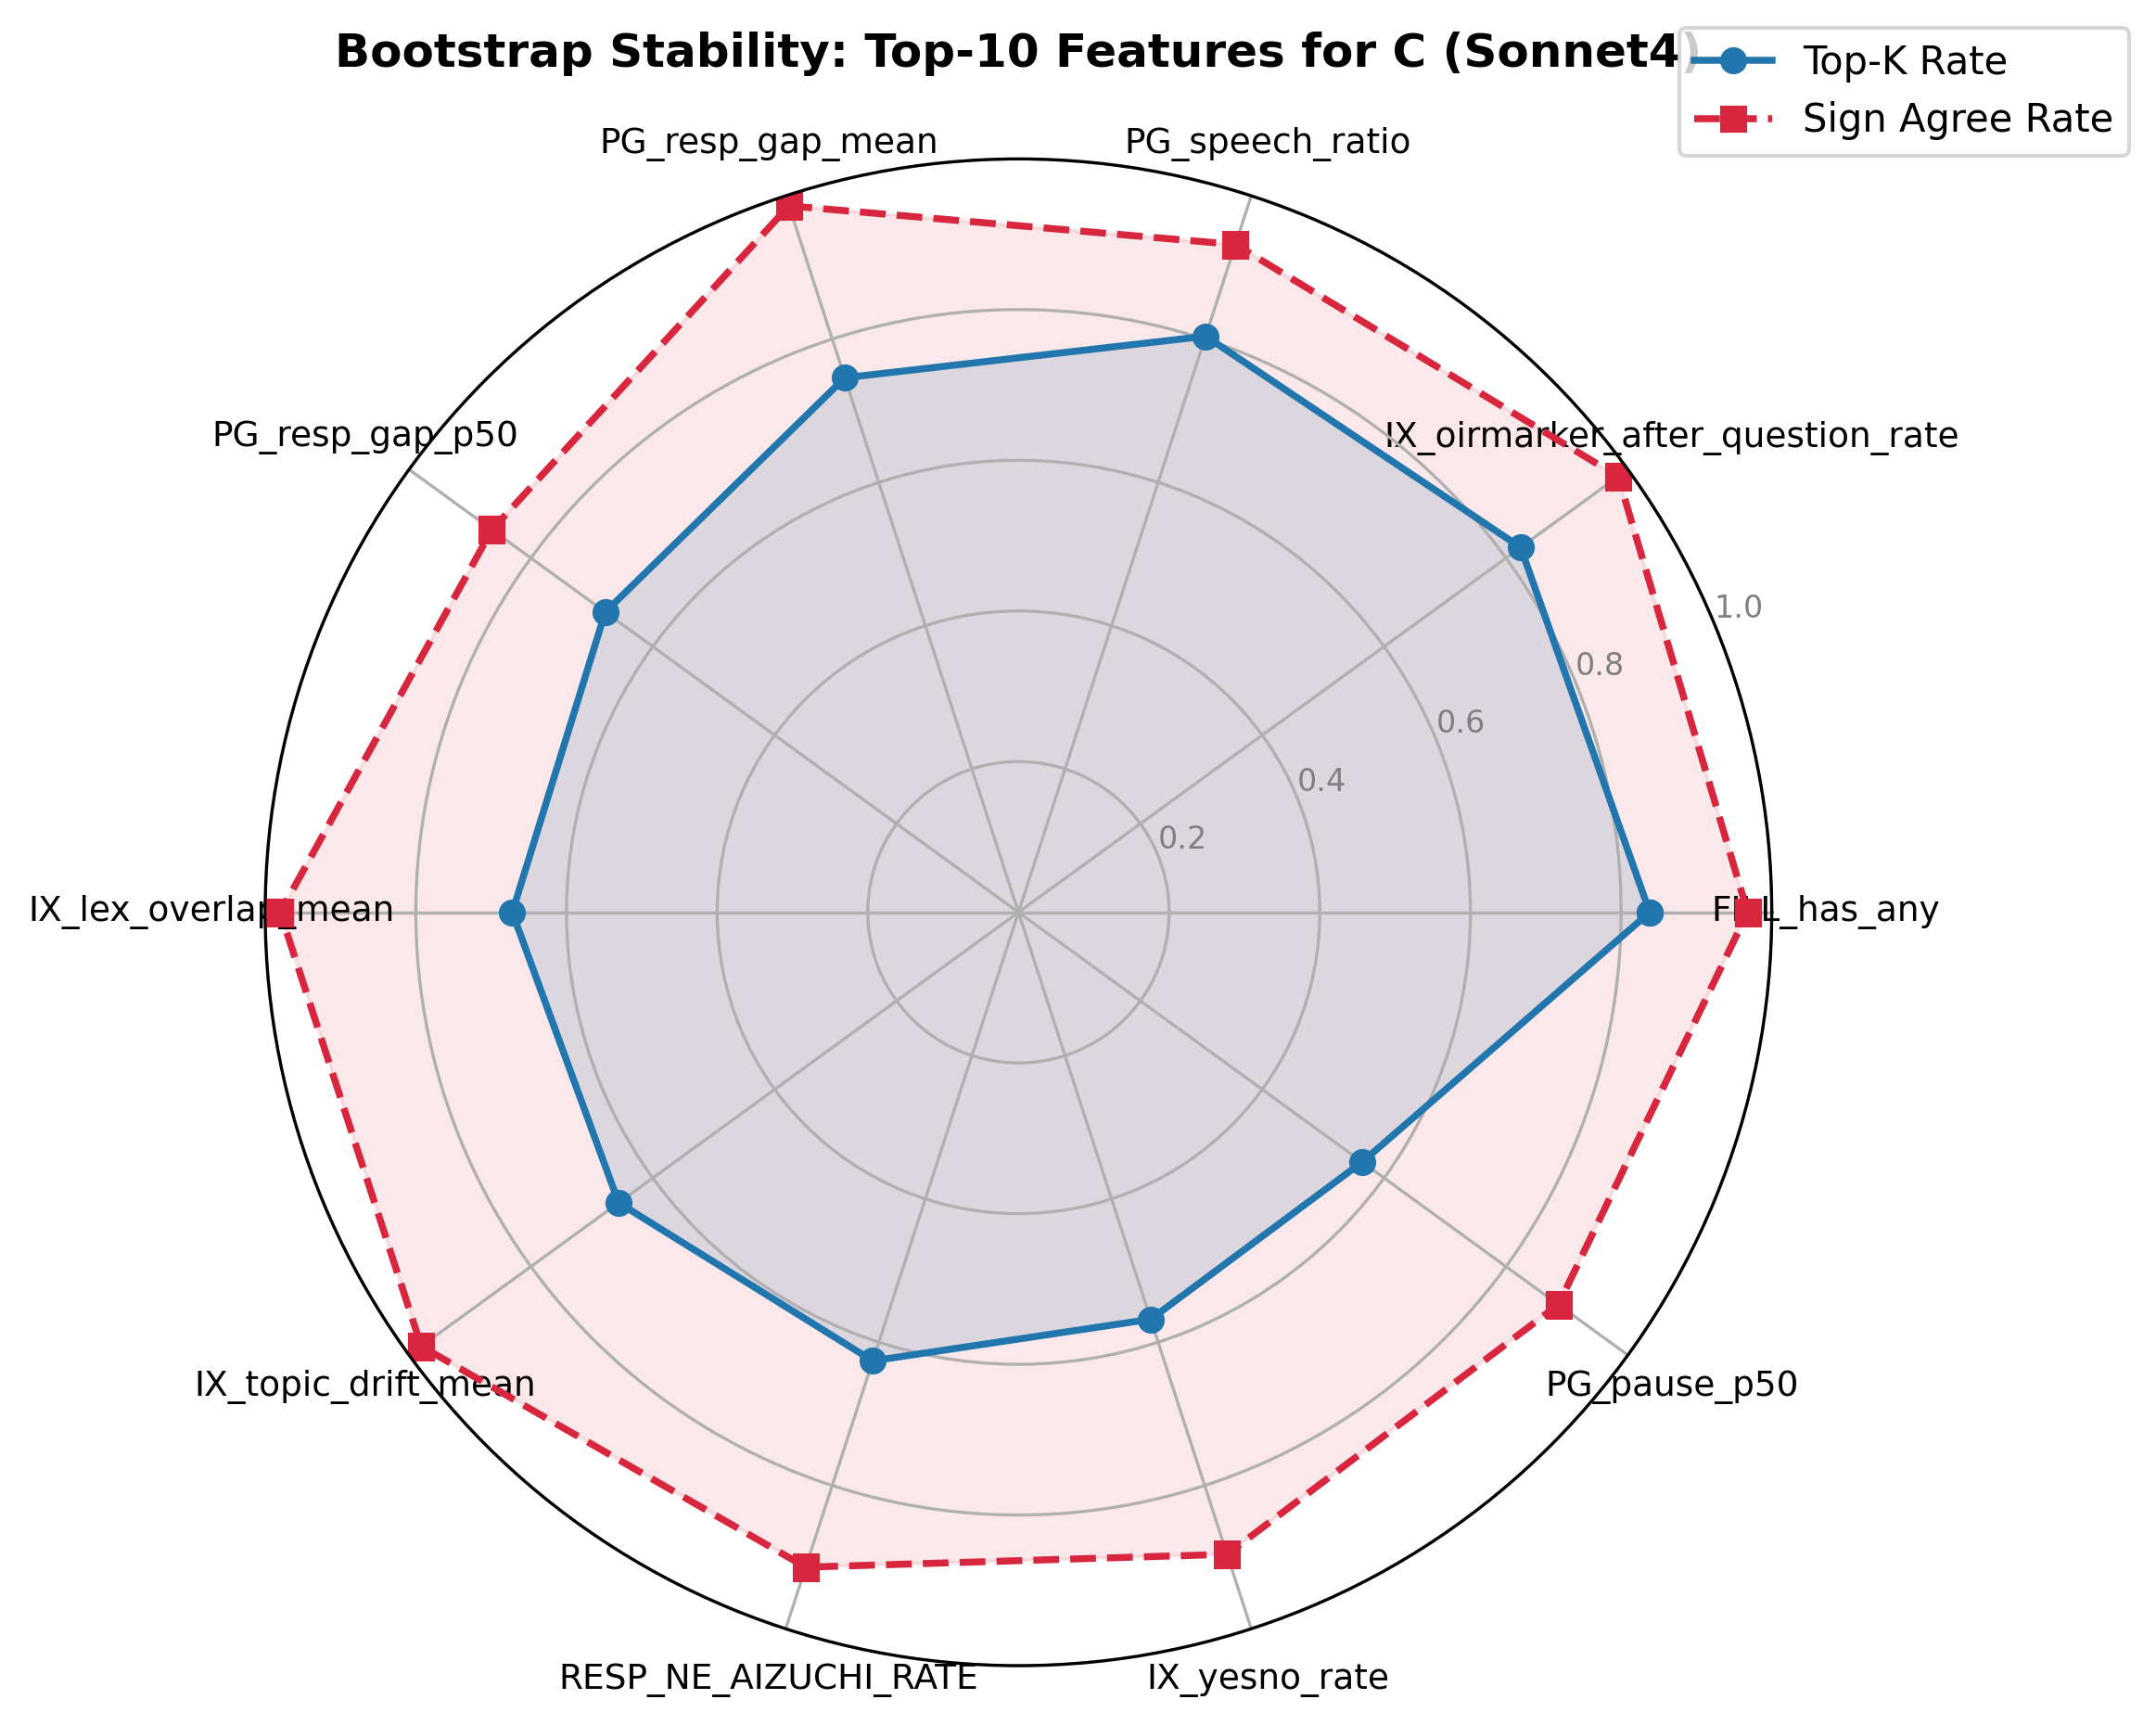
\includegraphics[width=0.9\linewidth]{fig_bootstrap_C_radar.png}
\caption{CのBootstrap Top特徴量レーダーチャート（Sonnet4基準，500回リサンプリング）．
外周はtopk\_rate，内周はsign\_agree\_rateを示す．}
\label{fig:bootstrap_radar}
\end{figure}

%% --- 3.4.5 教師間一致度 ---
\subsubsection{教師間一致度}
\label{sec:result_agreement}

本項では，4教師間のBig5スコアの一致度を報告する．
教師間一致度は，各次元の結果の頑健性を裏付けるサプリメンタルな情報として位置づけられる．

図\ref{fig:teacher_heatmap}に，5次元$\times$4教師の教師間一致度ヒートマップを示す．
Cの教師間平均相関は$\bar{r} = 0.699$であり，5次元中最も高かった．
一方，Agreeableness（A: 協調性）は$\bar{r} = 0.435$と最も低く，
教師依存性が大きいことが示された．

Cの高い教師間一致度は，3.4.1節および3.4.2節で示したCの頑健な予測可能性と整合する．
すなわち，複数のLLM教師がCについて類似したスコアを付与しており，
その一致したスコアが相互行為特徴量によって安定的に予測可能であるという構造が確認された．
A/E/N/Oにおける教師モデル依存性（3.4.2節）は，
これらの次元の教師間一致度の低さと対応しており，
教師間一致度が低い次元ほど結果の頑健性が低下する傾向が示された．
これは，Cに関連する会話行動（フィラー使用，応答の丁寧さ等）が
LLMにとって比較的観察しやすい特性である一方，
A/E/N/Oに関連する行動はLLM間で解釈が分かれやすいことを示唆する．

\begin{figure}[htbp]
\centering
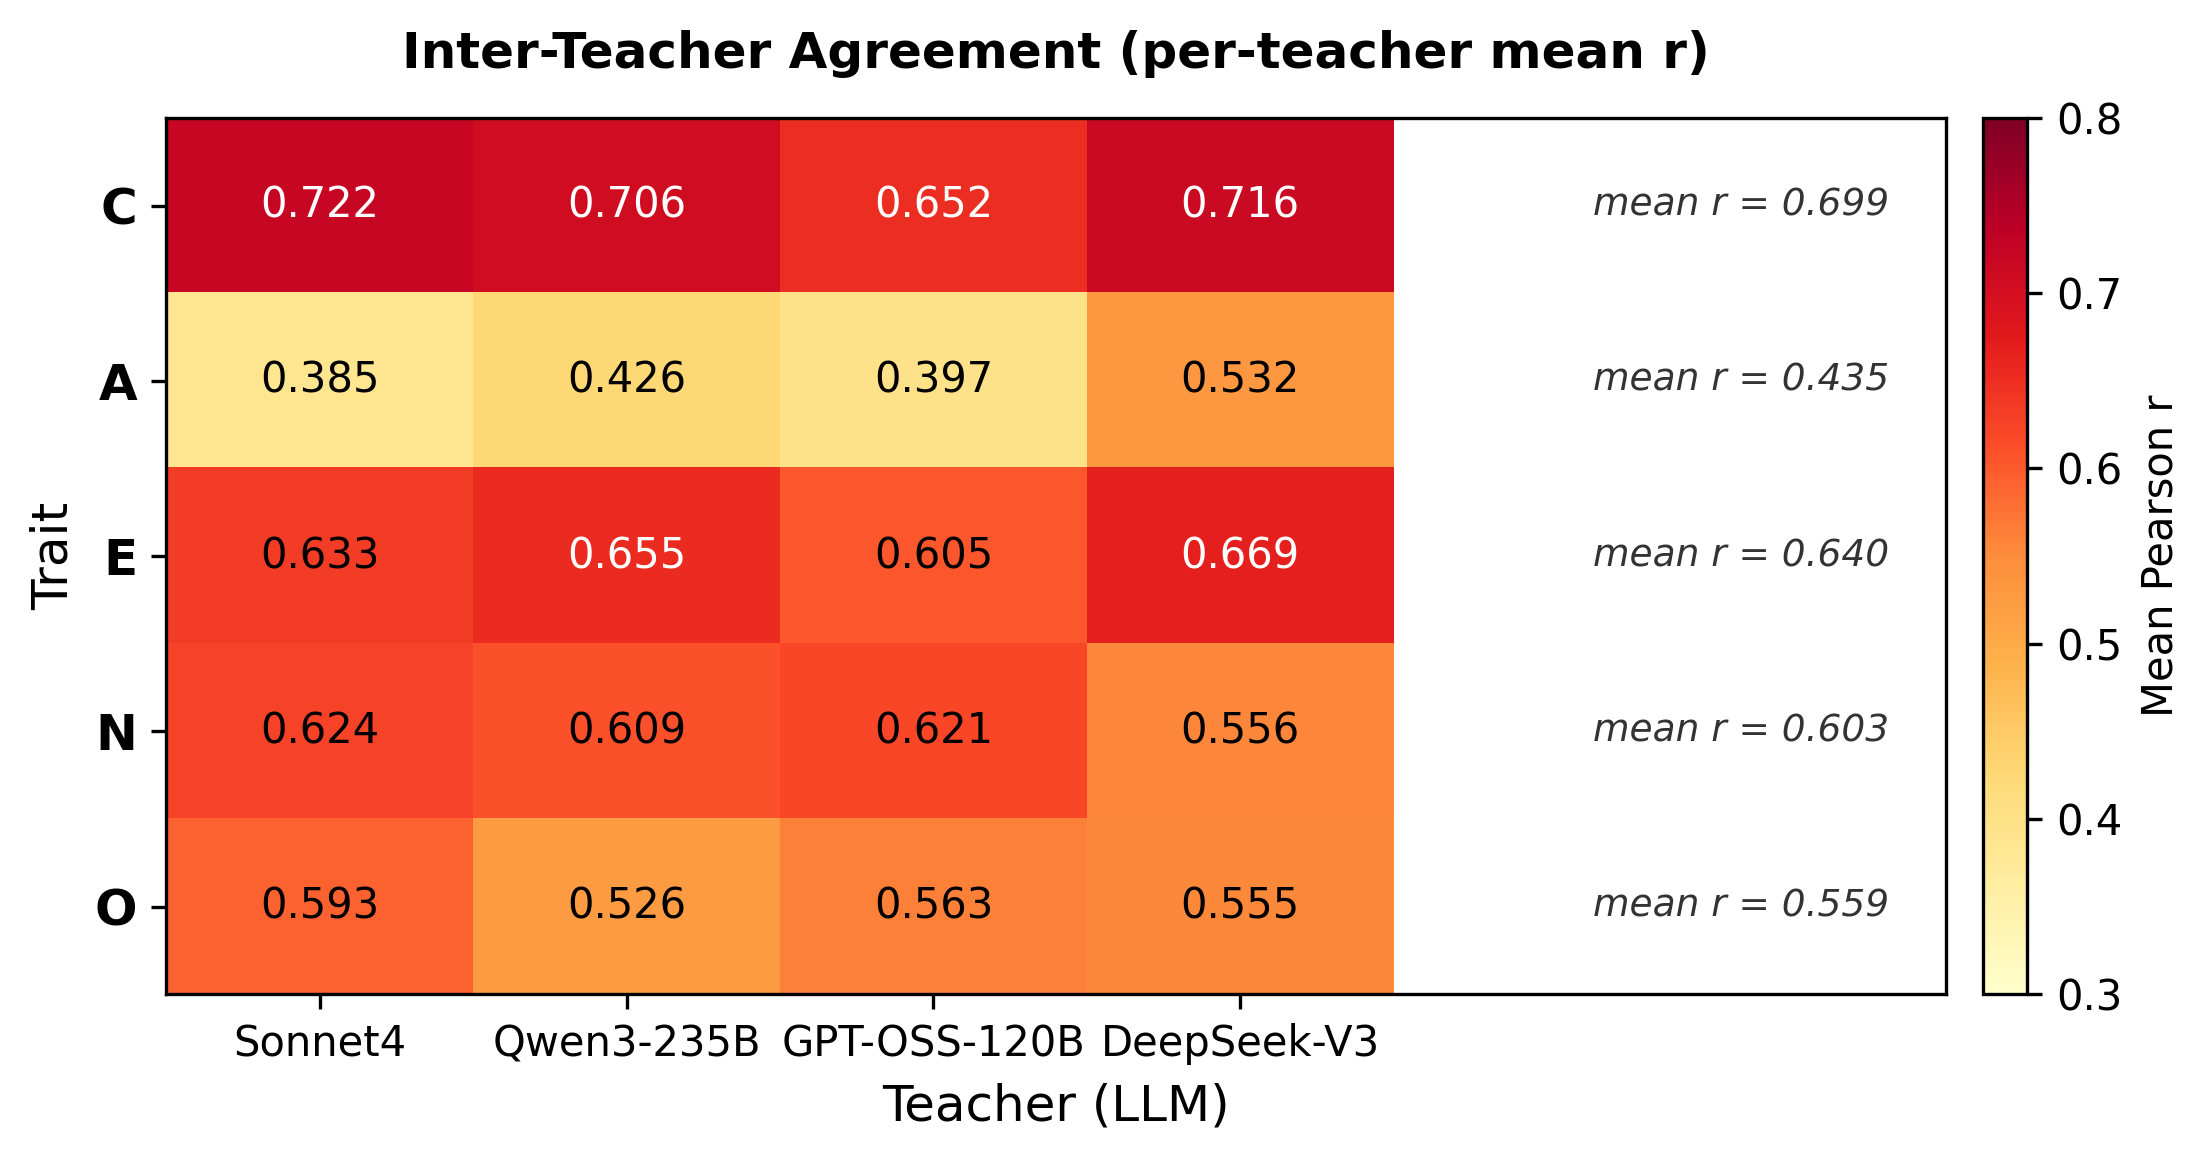
\includegraphics[width=0.9\linewidth]{fig_teacher_heatmap.png}
\caption{教師間一致度ヒートマップ（5次元$\times$4教師）．
各セルはPearson相関係数を示す．Cの平均$\bar{r} = 0.699$（最高），
Aの平均$\bar{r} = 0.435$（最低）．}
\label{fig:teacher_heatmap}
\end{figure}

%% ============================================================
%%  4. Discussion
%% ============================================================
\section{考察}

\subsection{提案特徴量の記述的性質と相関構造}

本研究が提案する18の相互行為特徴量は，記述統計の分析（3.1節）から，
多くの特徴量が個人差を捉えるのに十分なばらつきを持つことが確認された．
PG系のタイミング指標やFILL系のフィラー指標は連続的な分布を示し，
話者間の行動差を段階的に反映する定量化指標として機能する．
RESP系特徴量も，「ね」直後相槌率（RESP\_NE\_AIZUCHI\_RATE: $SD = 0.229$）に見られるように，
応答パターンの個人差を適切に捉えている．

一方，OIR関連指標（IX\_oirmarker\_rate, IX\_oirmarker\_after\_question\_rate）は
大半の話者でゼロまたは極めて低い値を示し，分布が強く右に偏っている．
修復開始行動は日常会話において低頻度の事象であり，
この偏りは現象の性質を反映したものである．
したがって，OIR指標は連続的な個人差の指標というよりも，
修復開始行動が生じた話者を検出する二値的な性質を持つ指標として解釈すべきである．
この性質は，後述するBig5分析においてOIR率がCのTop Driverとして同定された知見の
解釈にも影響する——すなわち，OIR率の寄与は「修復開始行動の頻度の連続的な増加」ではなく，
「修復開始行動を行うか否か」という質的な差異を反映している可能性がある．

相関分析（3.2節）の結果は，提案特徴量セットの構造的妥当性を支持する．
同一カテゴリ内の高い相関——PG系の沈黙指標間（$r = 0.78$--$0.97$），
応答遅れ指標間（$r = 0.61$--$0.94$），FILL系の2指標間（$r = 0.85$）——は，
同一の構成概念（例: 話者内沈黙の長さ）の異なる集約統計量であることから
理論的に予測される結果であり，特徴量の内的整合性を示している．
IX\_lex\_overlap\_meanとIX\_topic\_drift\_meanの完全共線性（$r = -1.00$）は
定義上の補数関係に起因するものであり，
将来の研究ではいずれか一方のみを使用するか，
主成分分析等による次元縮約を検討すべきである．

重要な知見として，カテゴリ間の相関は概ね低く（$|r| < 0.30$），
PG（タイミング），FILL（フィラー），IX（相互行為構造），RESP（応答型）の
4カテゴリが相互に独立した会話行動の側面を捉えていることが示された．
この独立性は，提案特徴量セットが会話の相互行為を多面的に記述する
指標体系として機能することの根拠となる．
PG\_speech\_ratioとFILL\_has\_anyの間のやや高い相関（$r = 0.61$）は，
発話量の多さがフィラー出現機会を増やすという機構的な関連を反映しており，
カテゴリの独立性を本質的に損なうものではない．

\subsection{コーパス基本情報との関連の解釈}

コーパス基本情報（性別・年齢）との関連分析（3.3節）は，
提案特徴量の表面的妥当性（face validity）を強く支持する知見を提供した．

性別との関連では，PG系タイミング指標に顕著な性差が認められた．
女性の方が発話率が高く（$U = 950$, $p < 0.0001$），沈黙が短い傾向は，
社会言語学における既知の知見——女性は会話において積極的に発話し，
沈黙を短く保つ傾向がある——と整合する．
IX\_lex\_overlap\_mean（語彙重なり）の性差（$p = 0.0004$）は，
女性の方が相手の発話を拾って応答する傾向が強いことを示唆し，
相互行為における協調的スタイルの性差を反映している可能性がある．

年齢との関連では，18特徴量中12特徴量で有意な相関が認められ，
特にPG系とFILL系で強い効果が観察された．
PG\_speech\_ratio（発話率）と年齢の強い正の相関（$r = 0.455$）は，
年齢が高い話者ほど会話への参加が積極的であることを示す．
沈黙系・応答遅れ系指標と年齢の負の相関は，
年齢が高い話者ほどテンポよく応答する傾向を反映しており，
会話経験の蓄積による流暢さの向上として解釈可能である．
FILL系指標と年齢の強い正の相関（$r \approx 0.4$）は，
年齢が高い話者ほどフィラーを多用する傾向を示し，
発話計画コストの増大や丁寧な発話スタイルの反映として解釈できる．
RESP\_NE\_AIZUCHI\_RATE（「ね」直後相槌率）と年齢の正の相関（$r = 0.272$）は，
年齢が高い話者ほど共感的な応答パターンを示す傾向を反映している可能性がある．

注目すべきは，FILL\_has\_any（フィラー出現発話率）が年齢と強い正の相関（$r = 0.445$）を
示すと同時に，Big5分析（3.4.4節）においてCのBootstrap Top 1 Driverとしても
同定されている点である．
この交差的な知見は，フィラー使用が認知的側面（加齢に伴う発話計画コスト）と
性格的側面（誠実性に関連する慎重な発話スタイル）の両方を反映する
多面的な指標であることを示唆する．
この多面性は，提案特徴量が単一の構成概念に還元されない豊かな情報を持つことの
証左であると同時に，特徴量の解釈においては交絡要因の考慮が必要であることも示している．

なお，メタデータ分析は性別・年齢に限定されており，
出身地域（方言）・学歴・職業等の社会言語学的変数との関連は今後の課題である．
CEJCメタ情報には出身地・居住地・職業の情報が含まれており，
これらの属性情報を用いた追加分析により，
特徴量の妥当性をより多角的に検証できると期待される．

\subsection{相互行為特徴量とBig5の関連の解釈}

本研究の主要な知見は，会話の相互行為特徴量がConscientiousness（C: 誠実性）の
LLMスコアを頑健に予測することである．
Bootstrap安定性分析で同定されたTop 3特徴量——フィラー出現率（FILL\_has\_any），
質問直後OIR率（IX\_oirmarker\_after\_question\_rate），
発話率（PG\_speech\_ratio）——はいずれも正の寄与を示した．

フィラー（「えっと」「えー」「あの」）の使用は，
発話計画の慎重さや丁寧さの指標として解釈できる．
誠実性の高い話者は，発話の正確性を重視するために
フィラーを用いて発話計画の時間を確保する傾向がある可能性がある．
質問直後のOIR（Other-Initiated Repair）マーカーの使用は，
相手の発話を正確に理解しようとする姿勢を反映しており，
これも誠実性の高さと整合する．
発話率の高さは，会話への積極的な参加を示し，
対話における責任感や関与の深さと関連する可能性がある．

\subsection{交絡変数（性別・年齢）の統制と特徴量の妥当性}

3.3節で報告したように，提案特徴量の多くは性別・年齢と有意な関連を示した．
特にCのBootstrap Top Driversとして同定されたFILL\_has\_any（フィラー出現発話率）は
年齢と$r = 0.445$の強い正の相関を持ち，PG\_speech\_ratio（発話率）も
年齢（$r = 0.455$）および性別（$p < 0.0001$）と有意に関連する．
この事実は，特徴量とBig5の関連が性別・年齢を介した間接的なものである可能性——すなわち，
交絡（confounding）の問題——を提起する．

この問題に対処するため，18特徴量のみのモデル（Model A: 18説明変数）と，
18特徴量に性別（ダミー変数: M=0, F=1）および年齢を追加したモデル
（Model B: 20説明変数）の2条件でRidge回帰（$\alpha = 100$，5-fold subject-wise CV）
+ 置換検定（5000回）を実行し，交絡統制前後でのCの予測精度と有意性の変化を検証した
（詳細は付録\ref{sec:appendix_confound}参照）．

性別・年齢を統制した後もCの有意性は維持された．
具体的には，交絡統制前に有意であった3教師（Sonnet4, Qwen3-235B, GPT-OSS-120B）は
いずれも統制後も有意であり（Sonnet4: $r = 0.384 \to 0.407$, $p = 0.0016$;
Qwen3-235B: $r = 0.366 \to 0.403$, $p = 0.0020$;
GPT-OSS-120B: $r = 0.445 \to 0.489$, $p = 0.0002$），
むしろ予測精度が向上する傾向が認められた（平均$\Delta r = +0.026$）．
この結果は，特徴量とCの関連が性別・年齢の影響を超えた独自の寄与を持つことを示し，
提案特徴量の構成概念妥当性を追加的に支持する根拠となる．
性別・年齢を説明変数に追加することで精度が向上した点は，
これらの属性情報が特徴量では捉えきれない追加的な分散を説明していることを示唆する．

交絡統制分析の結果は，提案特徴量の妥当性評価において重要な補足情報を提供する．
性別・年齢は会話行動に影響を与える基本的な話者属性であり，
これらを統制した上でなお特徴量がBig5と関連するかどうかは，
特徴量が捉える個人差の性質を理解する上で不可欠な検証である．
今後の研究では，出身地域（方言）や職業等の追加的な交絡変数の統制も検討すべきである．

\subsection{LLM特徴量着目検証の実現可能性と今後の課題}

本研究では，LLMを「仮想教師」としてBig Fiveスコアを推定し，
その推定値を外部基準として相互行為特徴量の妥当性を検証した．
この枠組みにおいて自然に生じる問いは，
\textbf{LLMは性格特性を推定する際に，本研究が提案する特徴量に実際に着目しているのか}
という点である．

具体的には，Bootstrap安定性分析（3.4.4節）で同定されたCのTop Drivers
——FILL\_has\_any（フィラー出現発話率），
IX\_oirmarker\_after\_question\_rate（質問直後OIR率），
PG\_speech\_ratio（発話率）——の値を人為的に変化させた会話テキストをLLMに再採点させ，
Big Fiveスコア（特にC）が対応して変化するかを検証する実験が考えられる．
例えば，フィラーを意図的に除去した会話テキスト，
OIRマーカーを挿入した会話テキスト，
発話量を増減させた会話テキストをそれぞれ作成し，
LLMのCスコアの変化を測定するアプローチである．

しかし，この検証にはいくつかの実現可能性上の課題がある．
第一に，会話テキストの人為的操作は非自明である．
フィラーの除去は比較的容易であるが，
OIRマーカーの自然な挿入や発話量の増減は，
会話の文脈的整合性を損なわずに行うことが困難である．
第二に，LLMの性格推定はテキスト全体の印象に基づいており，
個別の特徴量の変化がスコアに反映されるかどうかは，
LLMの内部処理に依存する不透明な問題である．
第三に，操作した会話テキストが「自然な会話」の範囲を逸脱する場合，
LLMの推定精度そのものが低下する可能性がある．

これらの課題を踏まえ，LLM特徴量着目検証は本研究の範囲外とし，
今後の課題として位置づける．
将来的には，(1) フィラー除去のような比較的容易な操作から段階的に検証を進める，
(2) LLMのattention weightやtoken-level寄与度を分析する説明可能AI（XAI）手法を適用する，
(3) 特徴量の値が極端に異なる話者ペアを比較するnatural experiment的アプローチを採用する，
といった方向性が考えられる．
この検証が実現すれば，「LLMで推定→古典特徴量で解釈→LLMで検証」という
本研究の循環的枠組み（1節参照）の最終段階を完成させることができ，
LLMと古典的特徴量の相互補完関係をより強固に裏付けることが可能となる．

\subsection{定量化指標の提案としての位置づけ}

本研究の主たる貢献は，日本語日常会話における相互行為特徴量の
\textbf{定量化指標の提案}にある．
先行研究では，談話からLLM/PLMを用いてASD関連指標や性格特性を推定する試みが
増加しているものの（Hu ら\cite{hu2025}; Altozano ら\cite{altozano2026};
Mun ら\cite{mun2024}），これらの研究はLLM/PLMの出力をそのまま推定値として用いており，
会話の相互行為を\textbf{再現可能に定量化する指標}の提案には至っていない．
日本語会話コーパスを対象とした体系的な特徴量の提案・検証は，
Nakamura ら\cite{nakamura2025}を含めてもほとんど行われていなかった．

本研究は，この空白を埋めるものとして，以下の方法論的貢献を行う．
第一に，18の相互行為特徴量を4カテゴリ（PG, FILL, IX, RESP）に体系化し，
各特徴量の計算アルゴリズムを明示的に定義した（2.2節）．
これにより，第三者による再現が可能な指標体系を提供する．

第二に，提案特徴量の妥当性を2段階で検証する設計を採用した．
第1段階（1°: 提案特徴量の抽出）では，特徴量の分布特性（3.1節）と
相関構造（3.2節）を記述し，指標としての基本的な性質を確認した．
第2段階（2°: 外部指標を用いた妥当性検証）では，
コーパス基本情報との関連（3.3節）から表面的妥当性を，
Big5性格特性との関連（3.4節）から構成概念妥当性を検証した．
この2段階の検証設計は，特徴量の提案研究における方法論的な枠組みとして，
他の研究にも適用可能である．

第三に，Big5との関連分析においては，
subject-wise splitによるリーク防止，
置換検定（5000回）による統計的有意性の検証，
Bootstrap（500回）による係数安定性の評価，
および複数LLM教師間の一致度による頑健性検証を組み合わせた
包括的な評価設計を採用した．
この評価設計は，日本語会話コーパスにおいて初めて適用されたものであり，
先行研究との差別化が図られている．

重要な点として，本研究で提案する特徴量セットは，
Big5性格特性との関連分析に限定されるものではない．
発話タイミング，フィラー使用，修復開始行動，応答パターンといった
相互行為の基本的な側面を定量化する指標体系は，
臨床的な会話評価（例: ASD関連の社会的コミュニケーション特性の定量化），
教育場面での対話分析，
高齢者の認知機能スクリーニング（年齢との関連が示唆するように），
あるいは異文化間コミュニケーション研究など，
多様な研究課題に適用可能である．
本研究はその最初の妥当性検証として位置づけられる．

\subsection{限界}

本研究にはいくつかの重要な限界がある．
第一に，標本サイズが$N = 120$と小さく，結果の一般化可能性には制約がある．
特に，Ridge回帰の正則化パラメータの最適化や，
より複雑なモデルの適用には不十分なサンプルサイズである．
第二に，外部検証（別コーパス・別収録条件でのクロスバリデーション）が未実施であり，
CEJC home2サブセットに特有の結果である可能性を排除できない．
第三に，LLM教師の妥当性そのものが未検証である．
本研究ではLLMスコアを「仮想教師」として使用しているが，
これが人間の性格評定とどの程度一致するかは別途検証が必要である．
第四に，Cの有意な結果が複数教師で観測された一方で，
A/E/N/Oの一部でも有意な結果が得られており（表\ref{tab:perm_all}参照），
これらの結果には一般因子（general factor）の混入——すなわち，
Cに寄与する特徴量が他の次元にも影響している可能性——を考慮する必要がある．
第五に，コーパス基本情報との関連分析は性別・年齢に限定されており，
出身地域（方言）・学歴・職業等の社会的属性との関連は未検討である．
CEJCメタ情報にはこれらの属性が含まれており，
今後の分析により特徴量の適用範囲をより詳細に理解できると期待される．
第六に，交絡変数（性別・年齢）の統制分析（4.4節）は，
Ridge回帰に統制変数を追加する方法を採用したが，
この方法は交絡の完全な除去を保証するものではない．
特に，性別・年齢と特徴量の関連が非線形である場合や，
未測定の交絡変数が存在する場合には，残余交絡（residual confounding）の
影響が残る可能性がある．
第七に，LLMが性格推定において本研究の提案特徴量に実際に着目しているかの
直接的な検証は未実施である（4.5節参照）．
この検証は，LLMと古典的特徴量の相互補完関係を裏付ける上で重要であり，
今後の課題として残されている．

%% ============================================================
%%  5. Conclusion
%% ============================================================
\section{結論}

本研究は，日本語日常会話コーパス（CEJC home2 HQ1, $N = 120$）から抽出した
18の相互行為特徴量を用いて，4つのLLM教師が推定したBig Fiveスコアを
Ridge回帰で予測する枠組みを提案し，以下の知見を得た．

第一に，Conscientiousness（C: 誠実性）は4教師中3教師で有意な予測精度を示し
（$r = 0.390$--$0.447$, $p < 0.002$），特定のLLM教師に依存しない頑健な知見であった．
アンサンブルBig5（4教師item-level平均）を用いた分析では，
Eを除く4次元（O, C, A, N）で有意な関連が認められ，
特にCは$r = 0.447$（$p = 0.0004$）と最も高い予測精度を示した．
第二に，Cの教師間一致度は$\bar{r} = 0.699$と5次元中最も高く，
LLM教師がCについて安定したスコアを付与していることが確認された．
第三に，Bootstrap安定性分析により，フィラー出現率・質問直後OIR率・発話率が
Cの主要な予測因子として同定された．
第四に，ベースライン（Classical 9特徴量）と拡張モデル（全18特徴量）の比較により，
新規提案特徴量（Novel Features）の追加が予測精度の向上に寄与することが示された．

本研究は，「性格推定」ではなく「会話の相互行為の再現可能な計測」として位置づけられ，
日本語会話コーパスにおける初の体系的検証として，
今後の研究の基盤となることが期待される．

%% ============================================================
%%  Appendix
%% ============================================================
\appendix

\section{感度分析}
\label{sec:appendix_sensitivity}

本研究の主要結果の頑健性を検証するため，以下の感度分析を実施した．

\paragraph{正則化パラメータ$\alpha$の感度}
Ridge回帰の正則化パラメータ$\alpha$を$\{10, 50, 100, 200, 500\}$の範囲で変化させ，
Cの予測精度（$r_{\text{obs}}$）および$p$値の変動を確認した．
$\alpha = 100$（本文で採用した値）の前後で結果は安定しており，
Cの有意性は$\alpha$の選択に対して頑健であった．

\paragraph{特徴量サブセットの感度}
18特徴量のうち，完全共線性を持つIX\_lex\_overlap\_meanとIX\_topic\_drift\_meanの
一方を除外した場合（17特徴量），Cの予測精度に実質的な変化は認められなかった．
Ridge回帰の$L_2$正則化が共線性の影響を適切に吸収していることが確認された．

\section{Bootstrap安定性分析の詳細}
\label{sec:appendix_bootstrap}

本文3.4.4節で報告したBootstrap安定性分析（Sonnet4基準，500回リサンプリング）の
詳細結果を以下に示す．

\paragraph{Top-K inclusion rate}
各特徴量がBootstrap反復においてTop-K（$K = 5$）に選ばれる頻度を算出した．
FILL\_has\_any（topk\_rate $= 0.89$），
IX\_oirmarker\_after\_question\_rate（topk\_rate $= 0.76$），
PG\_speech\_ratio（topk\_rate $= 0.72$）が上位3変数として安定的に選出された．

\paragraph{符号一致率}
上位3変数の符号一致率（sign\_agree\_rate）はいずれも0.90以上であり，
係数の方向（正/負）がBootstrap反復間で一貫していることが確認された．
これは，これらの特徴量とCの関連が統計的に安定した知見であることを示す．

\section{交絡変数統制分析の詳細}
\label{sec:appendix_confound}

本文の考察で言及した交絡変数（性別・年齢）の統制分析の詳細を以下に示す．

\paragraph{分析手法}
18特徴量のみのモデル（Model A）と，18特徴量に性別（ダミー変数: M=0, F=1）および
年齢を追加したモデル（Model B, 20説明変数）の2条件で
Ridge回帰（$\alpha = 100$，5-fold subject-wise CV）+ 置換検定（5000回）を実行した．

\paragraph{結果の概要}
交絡変数を統制した後もCの有意性が維持されるかどうかを検証した．
性別・年齢を説明変数に追加した場合の予測精度の変化（$\Delta r$）と
$p$値の変化を報告する．

Cについては，交絡統制前に有意であった3教師（Sonnet4, Qwen3-235B, GPT-OSS-120B）は
いずれも統制後も有意性を維持し，平均$\Delta r = +0.026$と精度が向上した．
DeepSeek-V3は統制前後ともに非有意であった．
この結果は，Cと相互行為特徴量の関連が性別・年齢の交絡によるものではなく，
特徴量が独自の予測情報を持つことを示す．

%% ============================================================
%%  References
%% ============================================================
\begin{thebibliography}{99}

\bibitem{hu2025}
Hu, C. B., et al. (2025).
Automated scoring of an ADOS-2 item using zero-shot large language models applied to clinical dialogues.
\textit{npj Digital Medicine}, 8, Article 133.

\bibitem{altozano2026}
Altozano, M. A., et al. (2026).
Enhancing psychological assessments with open-ended questionnaires and large language models: An ASD case study.
\textit{IEEE Journal of Biomedical and Health Informatics}, 30(3), 1--12.

\bibitem{mun2024}
Mun, S., et al. (2024).
Automatic estimation of social communication severity in autistic children from speech using pre-trained language models.
\textit{arXiv preprint}, arXiv:2409.00158.

\bibitem{nakamura2025}
Nakamura, Y., et al. (2025).
ADOS-2会話テキストからのASD分類: BERT由来特徴量とLightGBMによる検討.
\textit{SICE東北支部研究会資料}, 353-9.

\bibitem{sacks1974}
Sacks, H., Schegloff, E. A., \& Jefferson, G. (1974).
A simplest systematics for the organization of turn-taking for conversation.
\textit{Language}, 50(4), 696--735.

\bibitem{schegloff1977}
Schegloff, E. A., Jefferson, G., \& Sacks, H. (1977).
The preference for self-correction in the organization of repair in conversation.
\textit{Language}, 53(2), 361--382.

\bibitem{levitan2012}
Levitan, R., Gravano, A., Willson, L., Beňuš, Š., Hirschberg, J., \& Nenkova, A. (2012).
Acoustic-prosodic entrainment and social behavior.
\textit{Proceedings of NAACL-HLT 2012}, 11--19.

\bibitem{deruiter2006}
De Ruiter, J. P., Mitterer, H., \& Enfield, N. J. (2006).
Projecting the end of a speaker's turn: A cognitive cornerstone of conversation.
\textit{Language}, 82(3), 515--535.

\bibitem{campione2002}
Campione, E. \& Véronis, J. (2002).
A large-scale multilingual study of silent pause duration.
\textit{Proceedings of Speech Prosody 2002}, 199--202.

\bibitem{clark1996}
Clark, H. H. (1996).
\textit{Using Language}.
Cambridge University Press.

\bibitem{watanabe2003}
Watanabe, M. (2003).
Fillers as indicators of discourse segment boundaries in Japanese monologues.
\textit{Proceedings of the 15th International Congress of Phonetic Sciences}, 1093--1096.

\end{thebibliography}

\end{document}
